\chapter{Higgs Decays to Two Muons}\label{sec:hmumu}


The joint observation of the Higgs boson by ATLAS \cite{atlashiggs} and CMS \cite{cmshiggs} in 2012 initiated an era of studies of this particle and its interactions.
One of the reasons that the Higgs boson is interesting is that the Englert-Brout-Higgs (BEH) mechanism generates the mass of fermions by means of Yukawa couplings to the Higgs boson.
The most direct way to study these couplings is through the fermionic decay of the Higgs, described in Section \ref{sec:phenoHiggs}.
As the fermion branching ratios given Equation \ref{eqn:higgsDecayFermions} indicate, the Yukawa coupling is proportional to the fermion mass squared.
The $H\to\ttbar$ decay is kinematically forbidden because the top quark mass, $m_t\approx173$~GeV, exceeds the mass of the Higgs boson.
Consequently, the most probable decay path is to bottom quark pairs due to their large mass $m_b=4.2$~GeV. 
Despite this, the $H\ttbar$ coupling can be measured through the ttH process described in Table \ref{tab:higgsProdDiagrams}.
The $Hb\bbar$ coupling was observed at the ATLAS experiment using the VH production channels \cite{atlasHbb}.
The next most massive fermion after the bottom quark is the tau lepton, with $m_\tau=1.8$~GeV, which has been studied by ATLAS \cite{atlasTauTau} and CMS \cite{cmsTauTau}.
% I don't want the thesis to be immediately out of date
Although the charm quark with follows with a mass $m_c=1.3$~GeV, the messy hadronization of final state proves difficult to identify and study.
Searches for $H\to c\cbar$ remain insensitive even to $Hc\cbar$ couplings $\sim100$ times the Standard Model expectation.
This leaves the muon and the $H\mm$ coupling, where the muon's mass of $\m_\mu=0.1$~GeV results in a challengingly small branching fraction.
However, unlike the case with the charm quarks, the final state of two muons is easily identified by a clear experimental signature.
The result is that the $H\mm$ is the third and most challenging Higgs Yukawa coupling that is feasible to study at ATLAS.

\begin{figure}[h!]
\captionsetup[subfigure]{position=b}
\centering
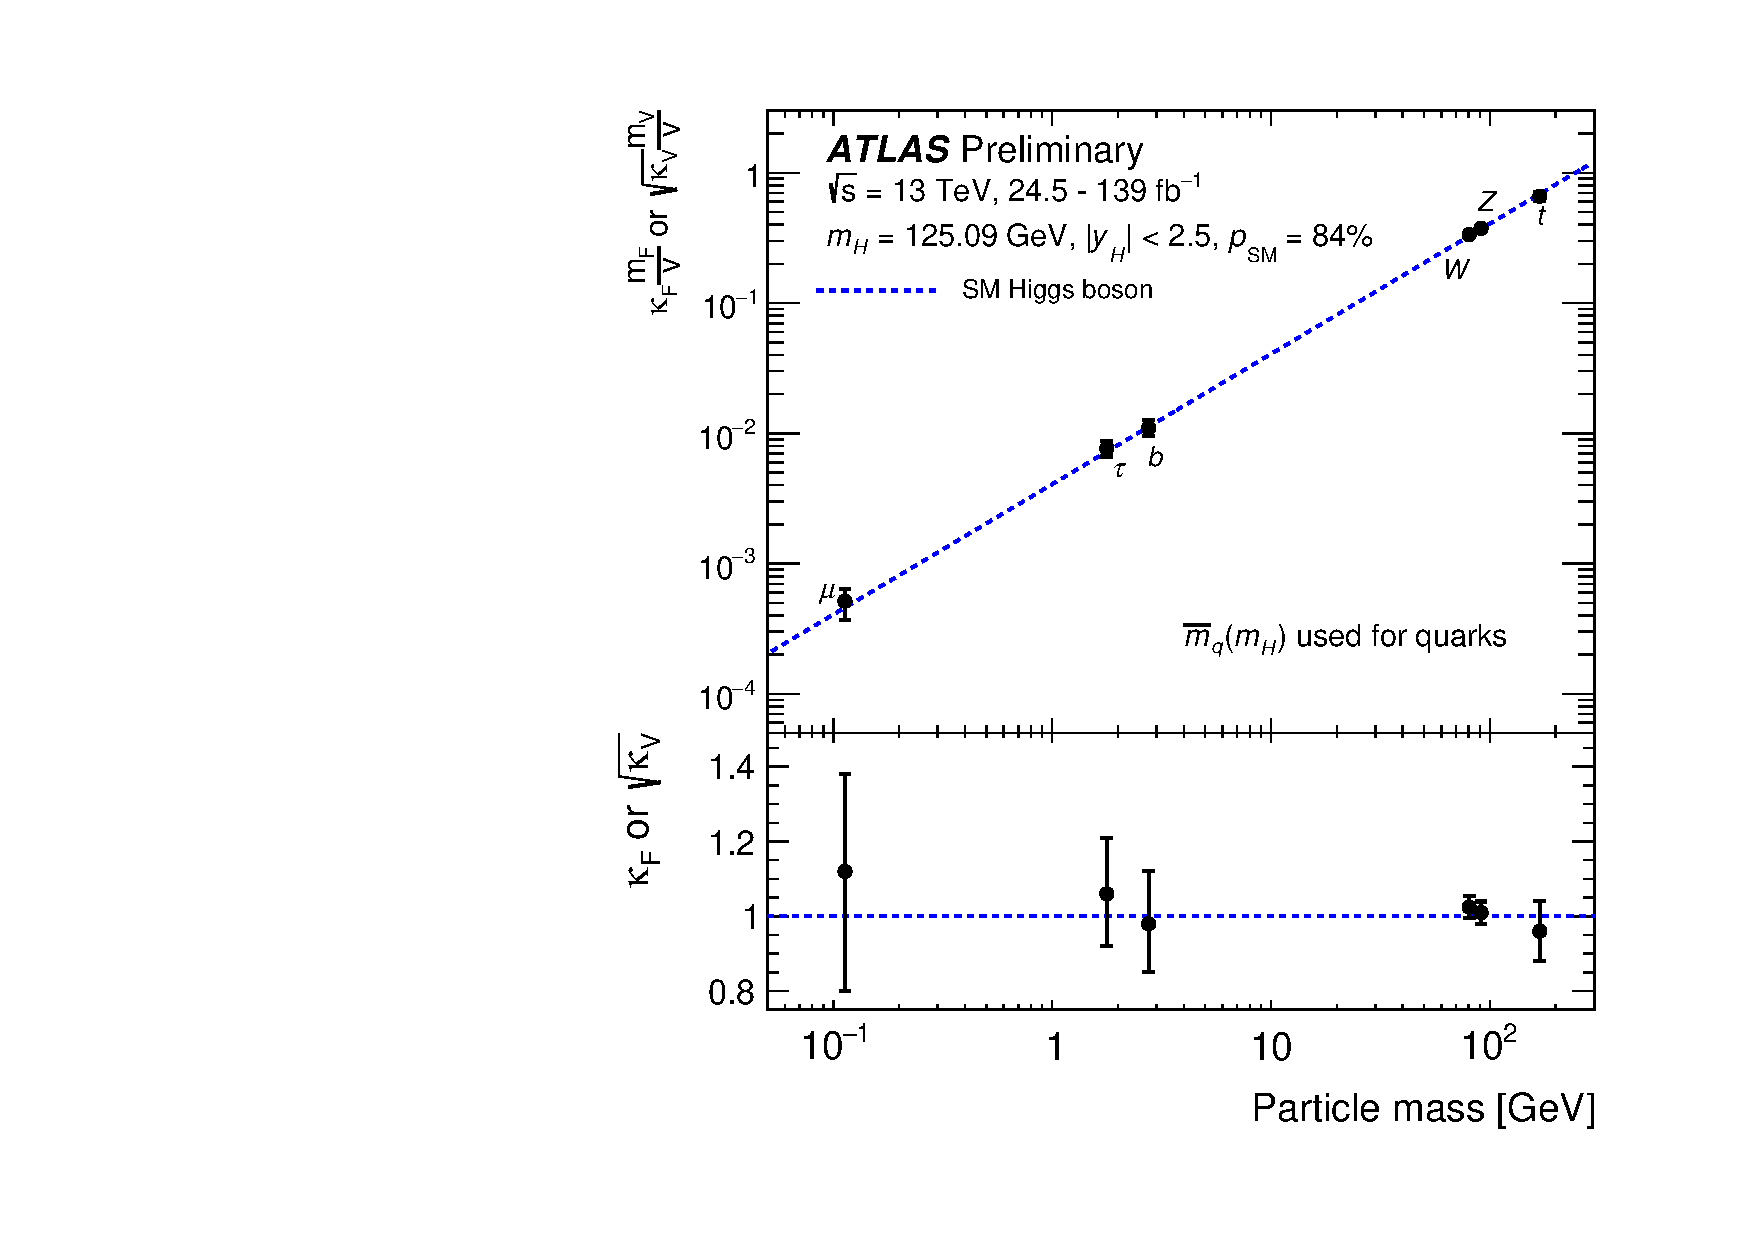
\includegraphics[width=0.7\textwidth]{figures/hmumu/massCouplingPlot.pdf}
\caption{Summary of ATLAS measurements of various fermion ($t$, $b$, $\tau$, and $\mu$) and gauge bosons. The plot shows the ``reduced coupling strength moderators'', where $\kappa$ is the deviation relative to the Standard Model prediction, compared to the particle's mass.
The SM prediction for both cases is also shown as a dotted line.
The contribution of this study appears in the bottom left corner of this plot. 
}
\label{fig:higgsMassCoupling}
\end{figure}

The $H\mm$ coupling also provides a unique opportunity as both the $Hb\bbar$ and $H\tautau$ couplings are to third-generation fermions.
This means that the \hmm measurement adds a valuable point to the global picture of Higgs couplings, as illustrated in Figure \ref{fig:higgsMassCoupling}.
Measuring this coupling provides a test of the Standard Model and also insight into the nature of the muon's mass.

Detecting the decays of Higgs to two muons is particularly challenging on two counts.
First, the Higgs branching fraction to muons is tiny ($2.18\times10^{-4}$).
Second, there is a sizeable irreducible dimuon background from Drell-Yan and Diboson processes.
Together these evoke the idiomatic needle-in-a-haystack to describe the search for \hmm.
It is only with the enormous number of events collected by ATLAS during the Run 2 data-taking campaign that it became feasible to perform this search.

%%%%%%%%%%%%% VH #################3

Of particular interest in this thesis are Higgs bosons produced through the VH production mechanisms.
These mechanisms are listed in Table \ref{tab:higgsProdDiagrams} as Higgs-strahlung and gluon-originated ZH.
They result in final states with a Higgs boson as well as an associated \W or \Z vector boson.
These events offer both a chance to look at a new, unstudied phase space, as well as a contribution to the overall sensitivity in the search for \hmm.
The events where the vector boson decays leptonically are particularly useful.
The additional leptons help differentiate VH events from the Drell-Yan background and provide kinematic information for further discrimination.

The cross-section of WH is 1.36~pb in center-of-mass collisions with energy $\sqrt{s}=13$~TeV, while the ZH cross-section is just 0.88~pb.

\begin{table}[htbp]
 \caption{Expected numbers of events from 139 fb$^{-1}$ $\sqrt{S}=13$ TeV data for WH and ZH. The first column shows the number of VH events, while the second column scales this by BR($H\to\mu\mu$) and the third column additionally multiplies by BR($V\to\ell\ell$) where $\ell$ is $e$ or $\mu$.}
 \begin{center}
\begin{tabular}{l c c c c}\toprule
% Production   & $H\to\mu\mu$ & $H\to\mu\mu,~V\to\ell\ell$ \\
Vector Boson  & VH & VH(\hmm) & VH(\hmm,~$^{W\to\ell\nu}_{Z\to\ll}$) \\
\midrule
V=\W & 189,040 & 41.5 & 9.14 \\
V=\Z & 122,320 & 26.9 & 1.83 \\
\bottomrule\end{tabular}
 \end{center}
\label{tab:vh-predict}
\end{table}

Studying \hmm with VH produced events introduces several challenges and opportunities.
First the tiny VH cross-section produces relatively few events to study.
Second is the question of how to use the new information from the leptonic vector boson decay products to separate the background from diboson production processes.
This information is particularly important to remove diboson (ZZ and WZ) backgrounds.
% Techniques to address challenge
Careful choices are made in the selection criteria targeted at VH production in order to capture as many VH/\hmm events as possible.
A multivariate analysis (MVA) discriminant is used to take advantage of the kinematic information in the \W and \Z decays.
Steps must be taken to understand and to limit the level of bias that these techniques introduce to the results. 
This is necessary to avoid invalidating the final measurements. 

\begin{figure}[htpb]
  \centering
    % \centered{\begin{tikzpicture}
    % \begin{feynman}
    %     \vertex (qa){\(\qbar\)};
    %     \vertex [below right=of qa] (p1);
    %     \vertex [below left=of p1] (qb){\(q'/q\)};
    %     \vertex [right=of p1] (p2);
    %     \vertex [above right=of p2] (h){\(H\)};
    %     \vertex [below right=of p2] (v){\(W/Z\)};
    %     \diagram* {
    %     (qb) --[fermion] (p1) --[fermion] (qa),
    %     (p1) --[boson,edge label=\(W/Z\)] (p2),
    %     (v) --[boson] (p2) --[scalar] (h),
    %     };
    % \end{feynman}
    % \end{tikzpicture}} 

\centered{\begin{tikzpicture}\begin{feynman}[medium]
    \vertex (p1);
    \vertex [right=3.6em of p1] (p2);
    \vertex [above left=of p1] (qa){\(\phantom{q'/}\qbar\)};
    \vertex [below left=of p1] (qb){\(q'/q\)};
    \vertex [above right=of p2] (h){\(H\phantom{/Z}\)};
    \vertex [below right=of p2] (v){\(W/Z\)};
    \diagram* {
    (qb) --[fermion] (p1) --[fermion] (qa),
    (p1) --[boson,edge label=\(W/Z\)] (p2),
    (v) --[boson] (p2) --[scalar] (h),
    };
\end{feynman}
\end{tikzpicture}} 
  \caption{VH production originating from quarks}
    \label{fig:vh-prod}
\end{figure}

The VH production mechanisms, WH and ZH, exemplified in Figure \ref{fig:vh-prod}, are the third and fourth leading Higgs boson production mechanisms at the LHC.
The cross-section of WH is 1.36~pb in center-of-mass collisions with energy $\sqrt{S}=13$, while the ZH cross-section is just 0.88~pb.
The cross-section, combined with the branching ratio of \hmm, results in the number of expected events per 139 fb$^{-1}$ shown in the first column of Table \ref{tab:vh-predict}.
In addition to the quark originating ZH shown in figure \ref{fig:vh-prod}, gluon originating ZH events contribute $\approx10\%$ to the total ZH cross-section.

\begin{figure}[h!]
\captionsetup[subfigure]{position=b}
\centering
\subfloat[][]{{
    \feynmandiagram [small,baseline=(v.base),horizontal=a to v] {a[particle=\(W^\pm\)] --[boson] v --[fermion] b[particle=\(\ell^\pm\)], c[particle=\(\nu\)] --[fermion] v,};
}}
\hspace{3em}
\subfloat[][]{{
    \feynmandiagram [small,baseline=(v.base),horizontal=a to v] {a[particle=\(Z\)] --[boson] v --[fermion] b[particle=\(\ell^+\)], c[particle=\(\ell^-\)] --[fermion] v,};
}}
  \caption{Leptonic decays of the \W (a) and \Z (b) bosons.}
  \label{fig:vh-decay}
\end{figure}

The search for \hmm is conducted in several categories of phase space defined based on the kinematics of the event.
Two inclusive categories are defined first: a 4-lepton selection targeting ZH produced events and a 3-lepton selection optimized for WH produced events.
These target leptonic ZH events with $\mu\mu\mu\mu$ or $ee\mu\mu$ final states, and leptonic WH events with $\mu\nu\mu\mu$ or $e\nu\mu\mu$.
In the case of leptonic decays of the \W, only the charged lepton is reconstructed, while a neutrino may be inferred from the scale and direction of missing transverse energy \met.
A further set categories are derived from these inclusive categories.
In the case of the 3-lepton selection, two sub-selections are defined with high WH yields and low background yields.
In the case of the 4-lepton selection, one high purity sub-selection is defined.
The delimitation of these exclusive categories from within the inclusive selections is based on the MVA discriminant.
This MVA is a function that maps various kinematic variables calculated from each event onto a spectrum related to the likelihood that an event is produced by a VH mechanism. 
The search is performed in the dimuon invariant-mass spectrum across these two inclusive and three exclusive categories.
A combination is performed using an additional seventeen categories that target other Higgs production mechanisms listed in Table \ref{tab:higgsProdDiagrams}.
The observations of this analysis were made public in June 2020 \cite{atlasHmm}.

This chapter describes the search for \hmm using the VH production channels with the full Run 2 dataset collected by ATLAS.
Section \ref{sec:hmmEvSel} describes the selection of data used for the search, followed by Section \ref{sec:hmmBdt} that describes the MVA based categorization.
Sections \ref{sec:hmmBkg} and \ref{sec:hmmSig} present the signal and background models, respectively.
Next Section \ref{sec:hmmSyst} discusses the systematic uncertainties used in the result.
Section \ref{sec:hmmStat} details the statistical analysis of the data.
Finally Section \ref{sec:hmmResults} presents the results of the analysis.

\section{\hmm Event Selection}\label{sec:hmmEvSel}

The search for \hmm is concerned with events containing at least two muons.
This section details the event selection, data, and simulation used in the analysis.

\subsection{Event Selection}\label{sec:hmmEv}

All data events are required to pass several criteria before they are considered for analysis.
Events are considered only if they were recorded while the ATLAS detector was in full operation.
The events meeting this requirement comprise the Good Run List, as summarized in Section \ref{sec:physData}.

Only a small fraction of the many events observed by ATLAS are useful to study. 
The trigger system decides on an event-by-event basis whether to record an event. 
Since \hmm events have muons in their final state, the analysis uses a trigger selection that requires at least one high-\pt muon.
The \pt threshold varies based on the year of data taking, depending on the trigger system's configuration.
In 2015 the minimum threshold was $\pt>20$~GeV, while in other years, it was $\pt>26$~GeV.
Muons with a \pt below 50~GeV are required to have isolated tracks in the ID to reduce the background event rate.
The efficiency of the trigger requirement is $\approx90\%$.

% Object selection
After passing the trigger requirement, the physics objects that comprise the event are tabulated.
The most important objects for leptonic VH \hmm are muons and electrons, but jets and \met are also used to reduce the background.
The definitions of the objects make use of identification and isolation requirements defined in Section \ref{sec:physObjects}.

The muons considered in an event meet the requirements listed in Table \ref{tab:hmmMuonObjSel}.
These can come from the Higgs decay, as well as the leptonic \W and \Z decays.
These are selected to be relatively inclusive due to the rarity of \hmm decays.
All four types of muons are used: CB, CT, ST, SA.
A particularly low \pt threshold of 6~GeV is selected with the four-muon ZH events in mind since one of the four muons often has a low \pt.

% Muons
\begin{table}[H]
        \caption{Muon selection criteria.}
    \begin{center}
        \begin{tabular}{ll}
            \toprule
            Type            &CB, CT, ST, SA\\
            Identification  &\code{Loose} \\
            Isolation       &\code{FixedCutPflowLoose}\\
            $\pt$           &$\pt > 6$~GeV\\
            $\eta$          &$|\eta| < 2.7$\\
            \multirow{2}{*}{Impact parameters}   &$|d_0^{\mathrm{BL}}/\sigma_{d_0^{\mathrm{BL}}}| < 3$\\
            &$|z_0^{\mathrm{PV}}\cdot \sin{\theta}| < 0.5$~mm\\
            \bottomrule
        \end{tabular}
        \label{tab:hmmMuonObjSel}
    \end{center}
\end{table}

The electrons are considered next, as these are produced by leptonic \W and \Z decays.
With a similar motivation to the muons, this selection is relatively lenient to maximize the selection's efficiency.
Several criteria are included to retain as many prompt electrons as possible while reducing the inclusion of fake electrons.
These are listed in Table \ref{tab:hmmEleObjSel}.

\begin{table}[H]
        \caption{Electron selection criteria.}
    \begin{center}
    %\footnotesize
        \begin{tabular}{ll}
            \toprule
            Identification    &\code{Medium} LH\\
            Isolation        &\code{FCLoose}\\
            $\pt$            &$\pt > 7$~GeV\\
            $\eta$            & $|\eta|<1.37$ or $1.52<|\eta|<2.47$ \\
            Quality            &Not "BADCLUSELECTRON"\\
            \multirow{2}{*}{Impact Parameters}    & $|d_0^{\mathrm{BL}}\ \mathrm{significance}|<5$ \\
            &$|z_0^{\mathrm{PV}} \cdot \sin{\theta}| < 0.5$~mm\\
            \bottomrule
        \end{tabular}
        \label{tab:hmmEleObjSel}
    \end{center}
\end{table}

Jets are reconstructed in order to remove background events from the VH selection.
The VH leptonic events are expected to produce small jet multiplicities.
Furthermore, jets are used to reduce the presence of ttH events in the selection, by vetoing events that a b-jet.
The criteria for jet selection are given in Table \ref{tab:hmmJetObjSel}.

\begin{table}[H]
    \caption{Jet selection criteria. Additionally, a combination of track-based variables are used suppress jets from other collisions in the same bunch crossing, called jet-vertex-tagger \cite{ATLAS-CONF-2014-018}.}
    \begin{center}
    %\footnotesize
    \begin{tabular}{ll}
        \toprule
        Algorithm        &AntiKt R=0.4 PFlow\\
        $\eta$            &$|\eta| < 4.5$    \\
        $\pt$            &$\pt > 25$~GeV for $|\eta| < 2.4$, $\pt > 30$~GeV for $2.4 < |\eta| < 4.5$ \\
        % JVT                & $\mathrm{JVT} > 0.59$ for $|\eta| < 2.4$ and 20~GeV$ < \pt < $120~GeV, $\mathrm{JVT} > 0.11$ for $2.4 < |\eta| < 2.5$ and 20~GeV$ < \pt < $120~GeV\\
        \bottomrule
    \end{tabular}
    \label{tab:hmmJetObjSel}
    \end{center}
\end{table}

Finally, the missing transverse momentum, \met, is calculated for the event.
The \met is calculated from the \pt of all reconstructed muons, electrons, and tracks not identified with one of these.
This serves as a proxy for the undetected neutrino from leptonic \W decays.

\begin{table}[htp]
\caption{Overlap removal criteria adopted for object selection, applied sequentially. The jet removal against muons is applied for jets satisfying $N_{Trk}(jet)<3$, or ($p_\mathrm{T}^{jet}/p_\mathrm{T}^{\mu}<2$ and $p_\mathrm{T}^{\mu}/\Sigma_{TrkPt}>0.7$)}
\begin{center}
\begin{tabular}{l l l l}
\toprule
Reject & Against & Condition \\
\midrule
\centered{Jet} & \centered{Electron} & \centered{$\Delta(e,\text{jet})R<0.2$} \\ 
\centered{Jet} & \centered{Muon} & \centered{$\Delta(\mu,\text{jet})R<0.2$} \\ 
\centered{Electron} & \centered{Electron} & \centered{lower \pt electron of shared track} \\ 
\centered{Electron} & \centered{Muon} & \centered{share track} \\ 
\centered{Electron} & \centered{Jet} & \centered{$0.2<\Delta(e,\text{jet})R<0.4$} \\ 
\centered{Muon} & \centered{Electron} & \centered{is calo-muon and shares track} \\ 
\centered{Muon} & \centered{Jet} & \centered{$0.2<\Delta(\mu,\text{jet})R<0.4$} \\
\bottomrule
\end{tabular}
\label{tab:hmmOr}
\end{center}
\end{table}

An overlap removal scheme is applied to avoid treating the same detector signature as multiple objects when two objects are reconstructed in close proximity.
This scheme removes objects according to the priorities listed in Table \ref{tab:hmmOr}.

Once the objects within an event have been determined, the next step is to identify events with objects matching the final state of leptonic VH processes.
All events are required at least one oppositely-charged muon pair that can serve as a candidate for \hmm.
Two parallel selections are carried out: 3-lepton events are selected targeting the WH process, while 4-lepton events are selected targeting the ZH process.

In events with two exactly two muons, these are required to be oppositely charged. In events with more than two muons, later charge requirements are applied, as described in table \ref{tab:hmmEv}. The leading $p_T$ muon is required to have $p_T>27$ GeV. The sub-leading $p_T$ muon is required to have $p_T>8$ GeV. The threshold for the sub-leading muon is lowered compared to the ggF/VBF selection to increase the signal yield efficiency. This change, in conjunction with the lower $p_T$ threshold for all muons and the loosening of the opposite charge requirement, increases WH signal yield by 16.9\% and ZH signal yield by 63\%.

Two selections are used to target VH production: a \emph{3-lepton} category that targets WH production where the W decays leptonically (electrons or muons), and a \emph{4-lepton} category that targets ZH production where the Z decays leptonically (electrons or muons).
The overall signal efficiency of the WH event selection is 45\%.
The signal efficiency of the ZH event selection is 37\%.
Both of the efficiencies are calculated with respect to the \W/\Z bosons decaying into electrons or muons.

The leptonic VH production does not produce many b-jets, in contrast to the top backgrounds and ttH signal production.
A veto of events containing b-jets helps reduce these backgrounds and also enhances the purity of the signal selection.
Section \ref{sec:expJets} describes how b-jets are identified with several working points that specify the efficiency of identifying a b-jet.
The loosest working point, 85\%, is selected based on its reaction of the background.
Figure \ref{fig:hmmBveto} illustrates signal and background yields in a comparison between vetoes using the 60\% and 85\% working points.
The looser 85\% working point constitutes a stricter veto, and it is seen to reduce the background yields in both the 4-lepton and 3-lepton selections.
The signal yields are not substantially affected.


\begin{figure}[h!]
\captionsetup[subfigure]{position=b}
\centering
\subfloat[][]{{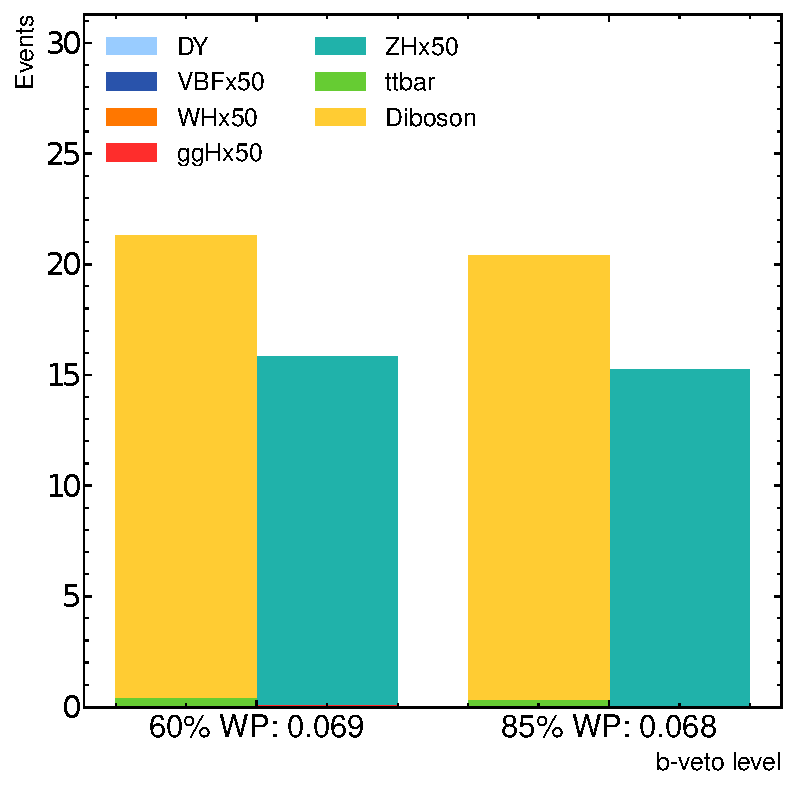
\includegraphics[width=0.4\textwidth]{figures/hmm/bveto/btag-4lep.pdf}}}
\subfloat[][]{{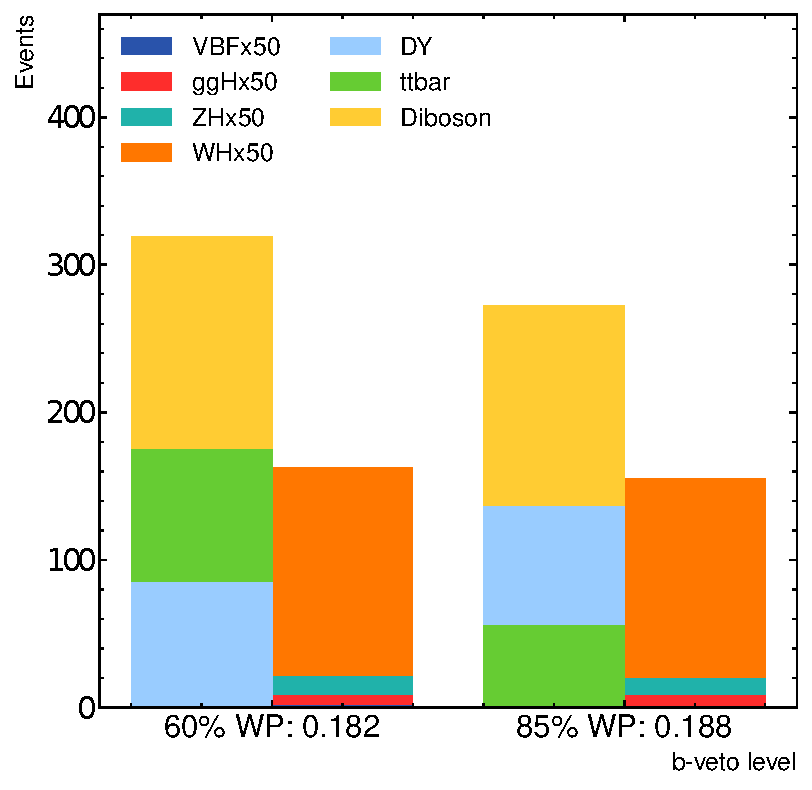
\includegraphics[width=0.4\textwidth]{figures/hmm/bveto/btag-3lep.pdf}}}
\caption{Illustration of the impact on signal and background yields of using different btag working points (WP) for the b-jet veto. This is shown for the 4-lepton selection (a) and 3-lepton selection (b). Each bar shown the number of simulated signal or background events passing the selection when using the WP marked on the x-axis. For both selections, using the looser 85\% WP reduces the background yields compared to the tighter 60\% WP. At the same time, the signal yield is relatively unchanged.}
\label{fig:hmmBveto}
\end{figure}

\begin{table}[ht!]
 \caption{Cutflow for 4-lepton and 3-lepton selection. Lepton pairs are opposite charge.}
 \begin{center}
\begin{tabular}{c c  c}\toprule
Step & 4-lepton & 3-lepton \\\midrule
1 & \multicolumn{2}{c}{No 85\% WP btag jets (b-jet veto)}           \\\midrule
2 & At least 4 leptons                                & Exactly 3 leptons\\\midrule
3 & ($N_{\mu^+}>$0 and $N_{\mu^-}>$0)                 & ($N_{\mu^+}>$0 and $N_{\mu^-}>$0) \\\midrule
4 & A dimuon pair $\exists\in$ [110,160] GeV                    & A dimuon pair $\exists\in$ [110,160] GeV \\\midrule
\multirow{2}{*}{5} & ($N_{\mu^+}>$1 and $N_{\mu^-}>$1) or              & ($N_{\mu^+}>$1 or $N_{\mu^-}>$1) or \\
  & ($N_{e^-}>$0 and $N_{e^+}>$0)                    & ($N_{e^-}>$0 or $N_{e^+}>$0)  \\\midrule
6 & $\nexists$ two Z$\to\mu\mu$ candidates                        & $\nexists$ Z$\to\mu\mu$ candidate  \\\midrule
7 & Higgs candidate $\in$ [110,160] GeV                  & Higgs candidate $\in$ [110,160] GeV \\\midrule
\multirow{2}{*}{8} & Kinematic cuts 27/15/8/6 GeV $>p_T$                    & Kinematic cuts 27/10/15(10) GeV $>p_T$ \\
  &                                                        & for $e(\mu)$ \\
\bottomrule\end{tabular}
 \end{center}
\label{tab:hmmEv}
\end{table}

The steps of the cutflow are shown in table \ref{tab:hmmEv}, which defines the 4-lepton and 3-lepton VH candidate categories.
This cutflow defines ``\Z candidates'' to be oppositely charged dimuon pairs an invariant-mass in $[80,105]$~GeV.
The selection of oppositely charged muons for the Higgs candidate, and of additional leptons for the \Z(\W) candidates is based on minimizing a $\chi^2$ calculation related to the invariant-mass (transverse-mass) and corresponding resolutions of the candidates.
This is shown in equations \ref{eq:hmmWhPairing} and \ref{eq:hmmZhPairing}.
Here, for each candidate pairing, $\chi^{2,\text{cand}}$ is calculated from the Higgs candidate mass $M_H^\text{cand}$.
For 4-lepton events, the \Z candidate mass $M_Z^\text{cand}$ is used, and for 3-lepton events the transverse-mass of the W candidate lepton and $E_T^\text{miss}$, $M_T^\text{cand}$, is used.
Only pairings with oppositely charged muons are considered for $M_H^\text{cand}$, while all oppositely charged same flavor pairs are considered for $M_Z^\text{cand}$.
Leptons of both flavors and charges are considered for $M_T^\text{cand}$.
The pairing with the smallest $\chi^{2,\text{cand}}$ is selected.

\begin{equation}
  \label{eq:hmmWhPairing}
  \chi^{2,\text{cand}}_{\W} = \frac{(M_H^\text{cand}-125\text{ GeV})^2}{(3.0\text{ GeV})^2} + \frac{(M_T^\text{cand}-70\text{ GeV} )^2}{(20\text{ GeV})^2}
\end{equation}

\begin{equation}
  \label{eq:hmmZhPairing}
  \chi^{2,\text{cand}}_{\Z} = \frac{(M_H^\text{cand}-125\text{ GeV})^2}{(3.0\text{ GeV})^2} + \frac{(M_Z^\text{cand}-91.1\text{ GeV} )^2}{(3.0\text{ GeV})^2}
\end{equation}

The $\chi^2$ pairing is used to improve the pairing efficiency.
Other pairing procedures were considered but were rejected based on their performance.
For example, in 4-muon events, selecting the highest $p_T$ opposite sign muon pair is 63.4\% less efficient than the $\chi^2$ pairing described above. 
Selecting the pair such that the \Z candidate is closest to the \Z mass is 8.7\% less efficient.

The cuts described in table \ref{tab:hmmEv} define two categories of events, 3-lepton and 4-lepton, which are referred to as inclusive categories in relation to the subsequent division into smaller categories.
The kinematic distributions of the leptons in these categories are illustrated in Section \ref{sec:hmmKine}.

\subsection{Simulation}\label{sec:hmmSim}

Simulated datasets play a central role in the search strategy.
All simulated datasets are scaled to match their corresponding cross-section \cite{higgsCross}.
First, the simulated background and signal datasets allow an exploration of the efficiency of various event selection criteria.
This eventually leads to the criteria listed in Table \ref{tab:hmmEv}.
Next, probability density distributions are constructed from simulated events that describe the probability to observe variables at a given value.
This is done both both for background and signal productions.
This allows the development of a multivariate discriminant function that separates signal and background events based on these variables.
% Simulated events are used at each step of this process: to determine the discriminant function with one set of simulated events and constrain the level of bias it may introduce with a second set of events.
% After this, an unrelated third set is used to estimate the rates of signal and background events, as a function of dimuon invariant mass, at different levels of discrimination.
The background rates as a function of \muu are used to measure systematic uncertainties and to validate the performance of several empirical background models.
The signal shape is used for these purposes as well, and most importantly, it provides the signal component in the hypothesis test performed on the observed data.
Finally, several theoretical and experimental variations on the signal shape are used to measure the impact of these uncertainties on the final result.

% Background ========================
The primary background production in the region of interest comes from Drell-Yan (DY), Diboson, and top production mechanisms described in section \ref{sec:phenoBkg}.
The dominant background mechanism, DY, primarily produces events with two leptons in the final state.
This is reduced through the requirement of more than two leptons in the event selection.
Processes involving $t\tbar$ and single-top production form a large background component as well.
Since the top quark always produces a bottom quark through decay, these backgrounds are mitigated by use of the b-jet veto in the event selection.
After this are diboson productions of $ZZ$ or $WZ$ with leptonic decays.
The diboson is topologically the most similar to the VH signal, making this the most challenging process to reject.
Diboson events are reduced with the help of a discriminant function based on several kinematic observables, but these events remain the dominant background after all selections are complete.

The DY simulations are generated with \sherpa 2.2.1 using the NNPDF3.0 PDF.
The DY \muu spectrum falls exponentially.
To generate sufficient numbers of high-mass events, these are simulated in ranges of $x$, where $x$ is the maximum of the mediator \pt and the scalar parton \pt sum, \httt.
These simulations are produced to NLO for diagrams, including fewer than three jets and LO for diagrams, including three or four jets.

The $t\tbar$ and single-top simulations are produced with \powheg v2 and the NNPDF3.0NLO PDF.
The mass of the top quark is set to $m_t=172.5$.
The $t\tbar$ cross section is calculated to NNLO using Top++2.0 \cite{Czakon:2011xx}.
The leading order $t\tbar$ Feynman diagrams are shown in Figure \ref{fig:phenoTtbar}.
The cross-sections of single-top production channels are calculated to NNLL accuracy following the standard procedure \cite{Kidonakis:2011wy, Kidonakis:2010ux}.
The leading order single-top Feynman diagrams are shown in Figure \ref{fig:phenoSingleTop}.
Different simulations are generated for $s$-channel and $t$-channel production through the exchange of a \W boson. A sample is produced for single-top production in association with a \W as well.

The final background simulations are composed of the diboson processes $WZ$ and $ZZ$ with leptonic decays.
These are produced with \sherpa 2.2.1 (for quark decays) and \sherpa 2.2.2 (for fully leptonic decays) and the NNPDF3.0 PDF.
Some number of fully or partially leptonic decays of the diboson final state are simulated in order to be considered as an additional background.
One set of simulations simulates $ZZ\to q\qbar\ll$ and $WZ\to q\qbar\ll$ events, while a second set simulates events with $\ll\ll$, $\ll\ell\nu$, and $\ll\nu\nu$ final states \cite{ATL-PHYS-PUB-2017-005}.
The purely leptonic $\ll\ll$ originates from two \Z decays.
This is the primary background in the 4-lepton categories and shares a very similar topology to ZH.
For completeness, the $ZZ$ decay to $\ll\nu\nu$ is simulated as well.
The production of $WZ$ $\ll\ell\nu$ is the primary background for several 3-lepton categories.
The leading order diboson Feynman diagrams are shown in Figure \ref{fig:phenoDiboson}.

% Signal simulations ========================
Signal simulations are produced based on the dominant Higgs production mechanisms listed in Table \ref{tab:higgsCrossSec}.
Most simulations are simulated with a Higgs mass set to 125~GeV using \powheg v2 and the PDF4LHC15 PDF. 
The exception is ttH, which is produced with \madgraph and the NNPDF3.0NLO PDF.
The precision ranges from NNLO in QCD for the ggF, to NLO for the VBF, VH, and ttH mechanisms.
The contribution of $gg\to ZH$ is simulated at LO.


\subsection{Kinematic Distributions}\label{sec:hmmKine}

The pre-cut categories defined in Section \ref{sec:hmmEv} are illustrated here with the aid of the simulated signal and background simulations.
The mass distributions are presented in Figure \ref{fig:hmmPrecutMassHists}.
These provide an illustration of the composition of the background and signal contributions to these categories, as well as the general agreement between data and simulation. 

\begin{figure}[h!]
\captionsetup[subfigure]{position=b}
\centering
\subfloat[][]{{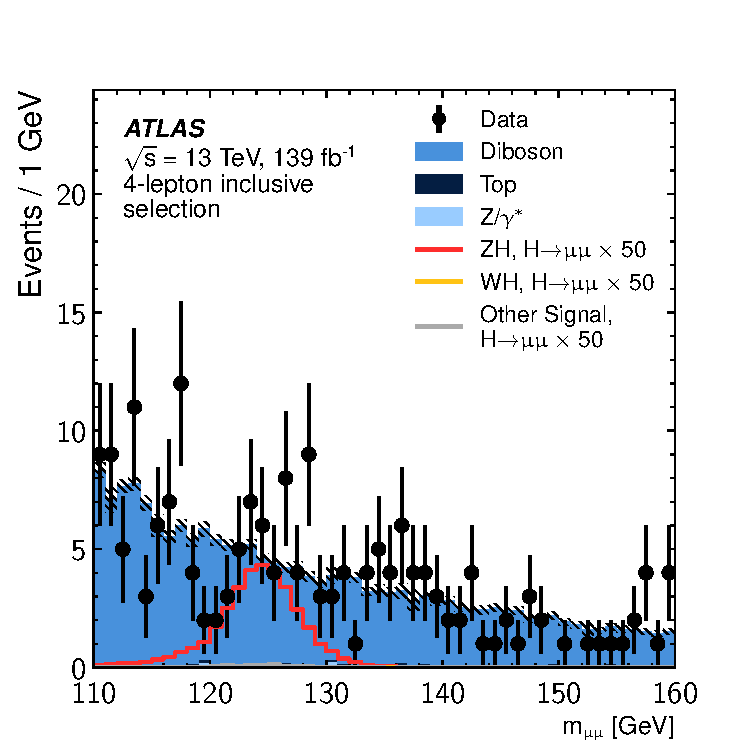
\includegraphics[width=0.5\textwidth]{figures/hmm/public/preCut/histo-4lep-muu.pdf}}} % public version of plots
\subfloat[][]{{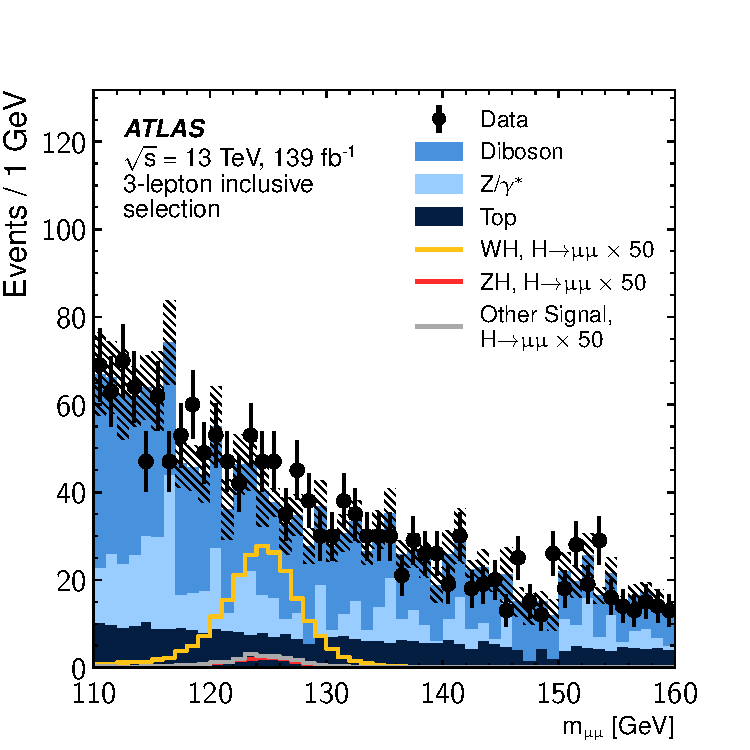
\includegraphics[width=0.5\textwidth]{figures/hmm/public/preCut/histo-3lep-muu.pdf}}}
% \subfloat[][]{{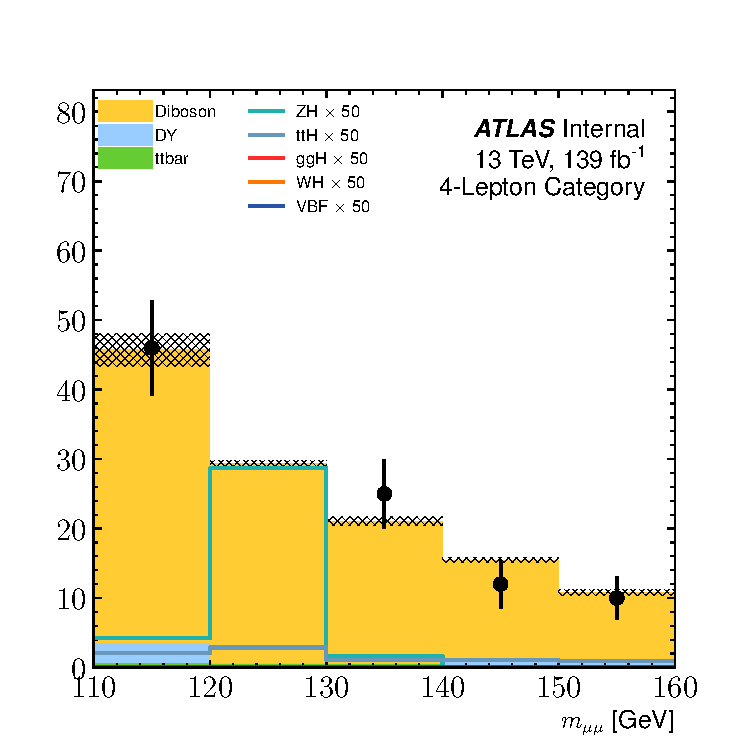
\includegraphics[width=0.5\textwidth]{figures/hmm/preCut/histo-4lep-muu.pdf}}}
% \subfloat[][]{{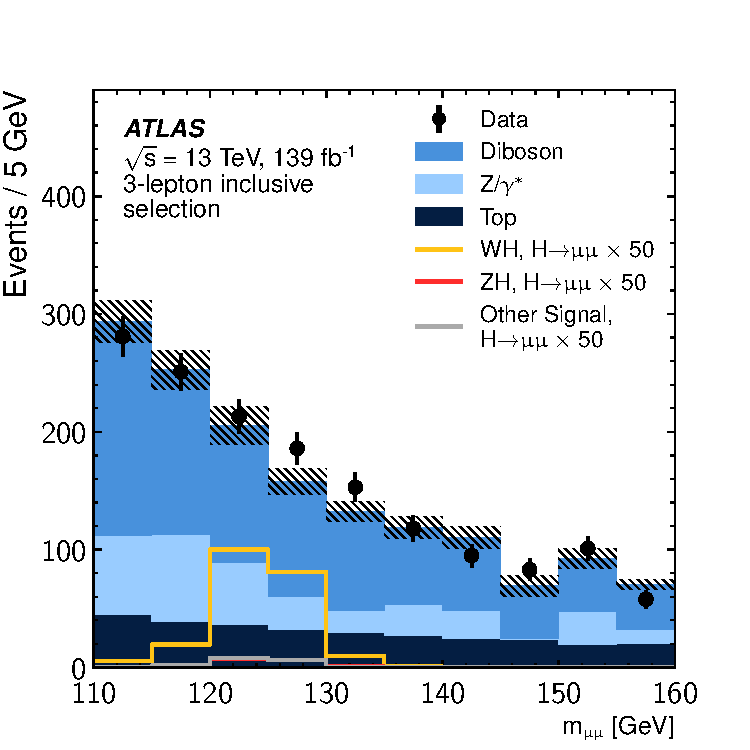
\includegraphics[width=0.5\textwidth]{figures/hmm/preCut/histo-3lep-muu.pdf}}}
\caption{Distributions of \muu in the 4-lepton (left) and 3-lepton (right) categories. The binning is adjusted based on the multiplicities of the categories. The signal distributions, shown in colored lines, are scaled by a factor of 50 for visibility.}
\label{fig:hmmPrecutMassHists}
\end{figure}

    
Other kinematic distributions ($p_T$, $\eta$, $\phi$) for the selected leptons are illustrated in Figures \ref{fig:hmmKineWhMuons} to \ref{fig:hmmKineZhLeps}.
The muon candidates for the Higgs are called $\mu^1$ and $\mu^2$ in descending order of $p_T$. 
Likewise, for the 4-lepton category, the selected leptons for the Z candidate are named $\ell^1$ and $\ell^2$ again in descending order of $p_T$.



\clearpage
\begin{figure}[htpb]
  \centering
  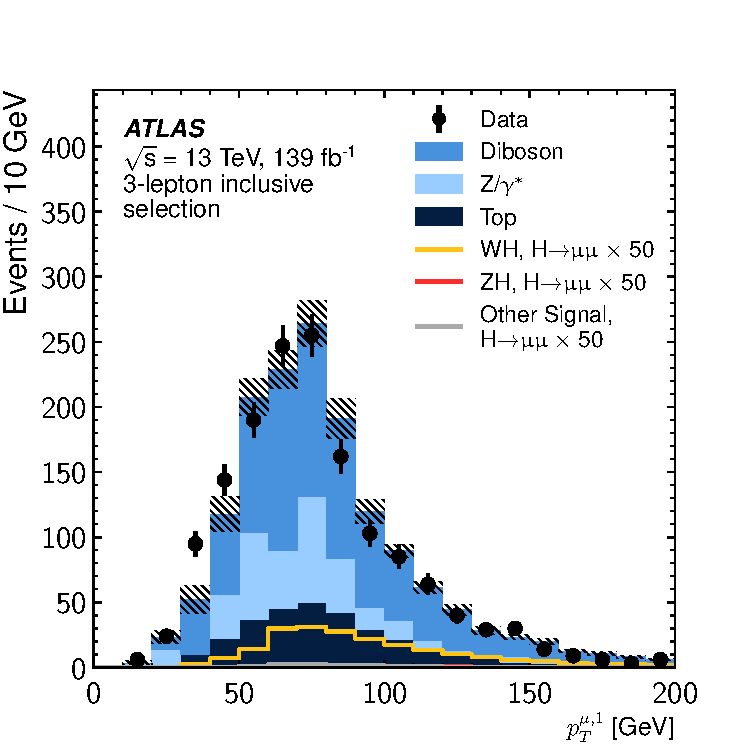
\includegraphics[width=0.4\textwidth]{figures/hmm/kinematics/histo-3lep-u1_pt.pdf}
  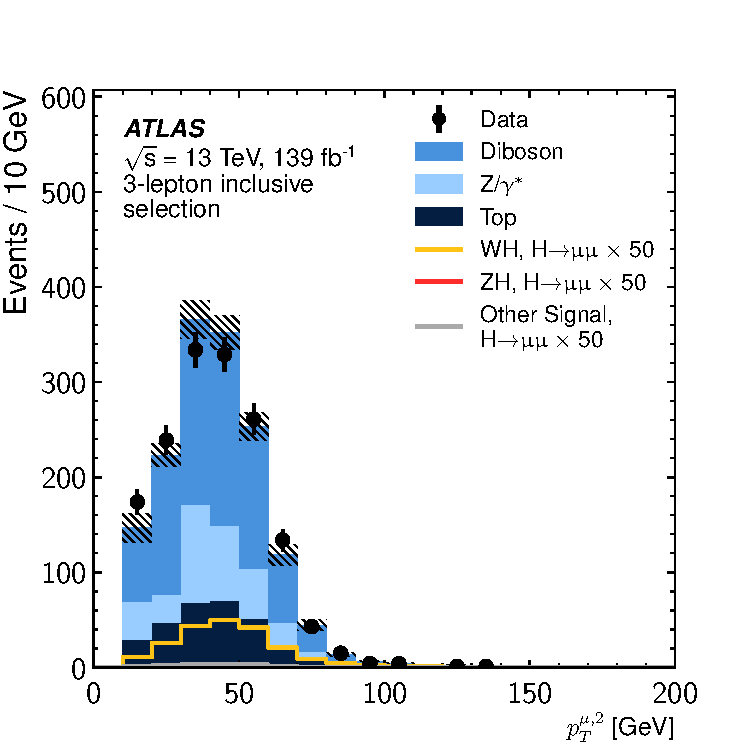
\includegraphics[width=0.4\textwidth]{figures/hmm/kinematics/histo-3lep-u2_pt.pdf}
  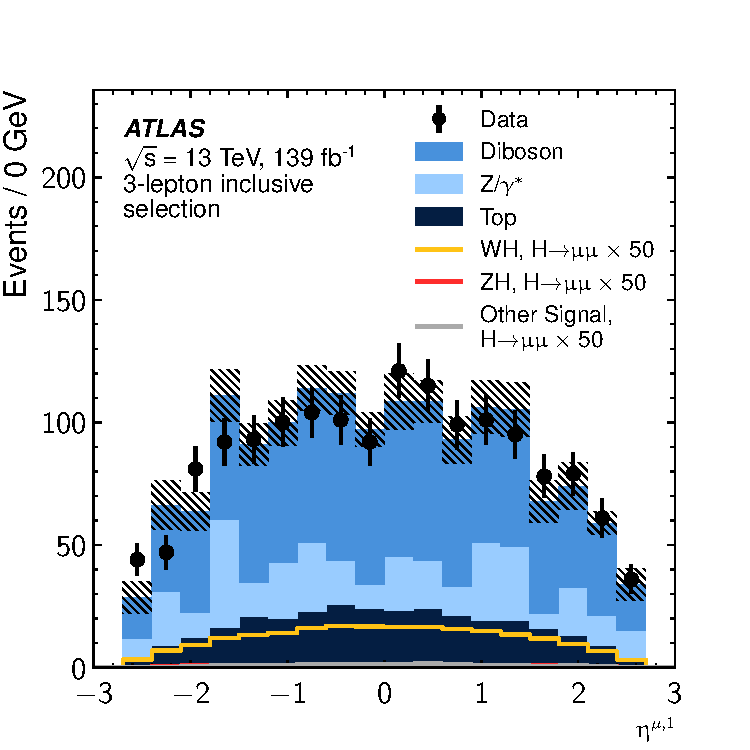
\includegraphics[width=0.4\textwidth]{figures/hmm/kinematics/histo-3lep-u1_eta.pdf}
  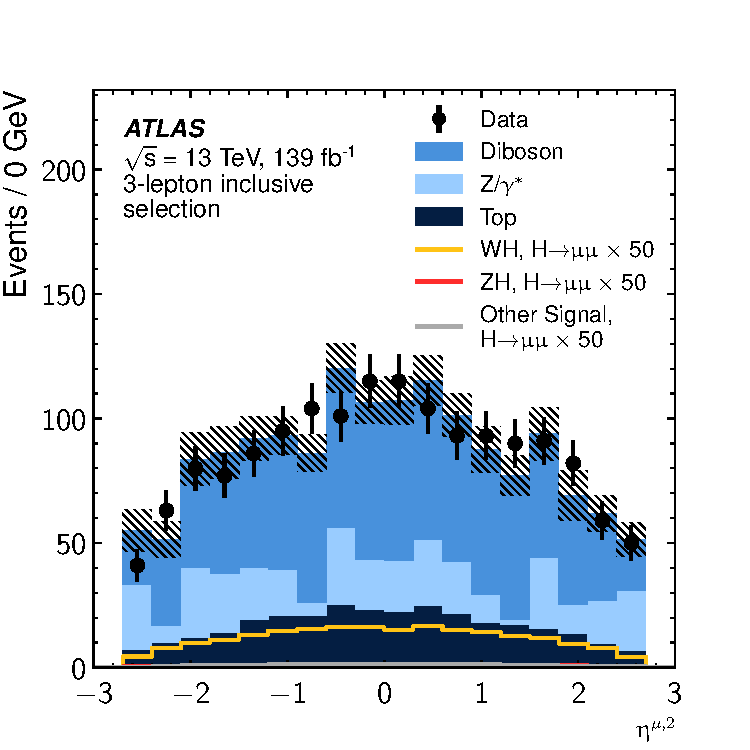
\includegraphics[width=0.4\textwidth]{figures/hmm/kinematics/histo-3lep-u2_eta.pdf}
  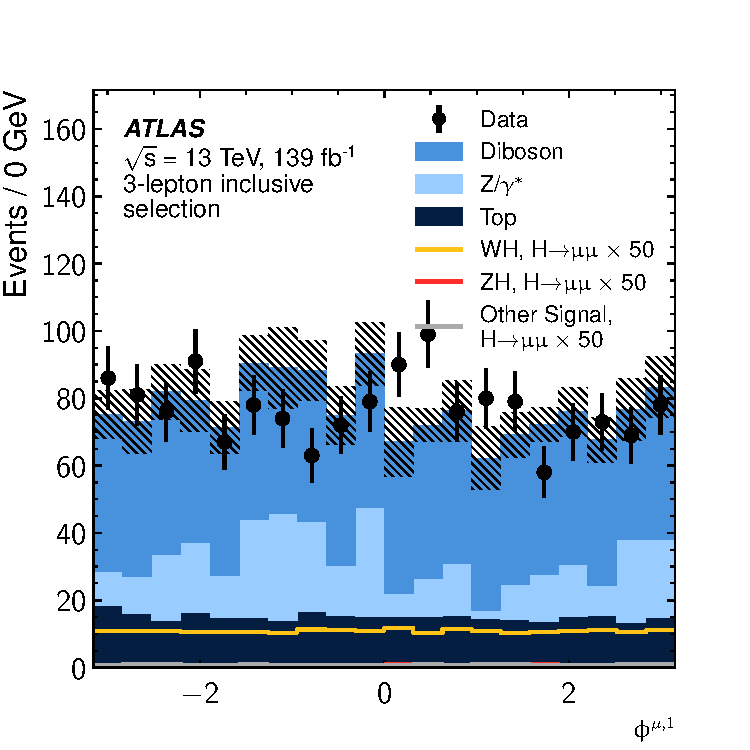
\includegraphics[width=0.4\textwidth]{figures/hmm/kinematics/histo-3lep-u1_phi.pdf}
  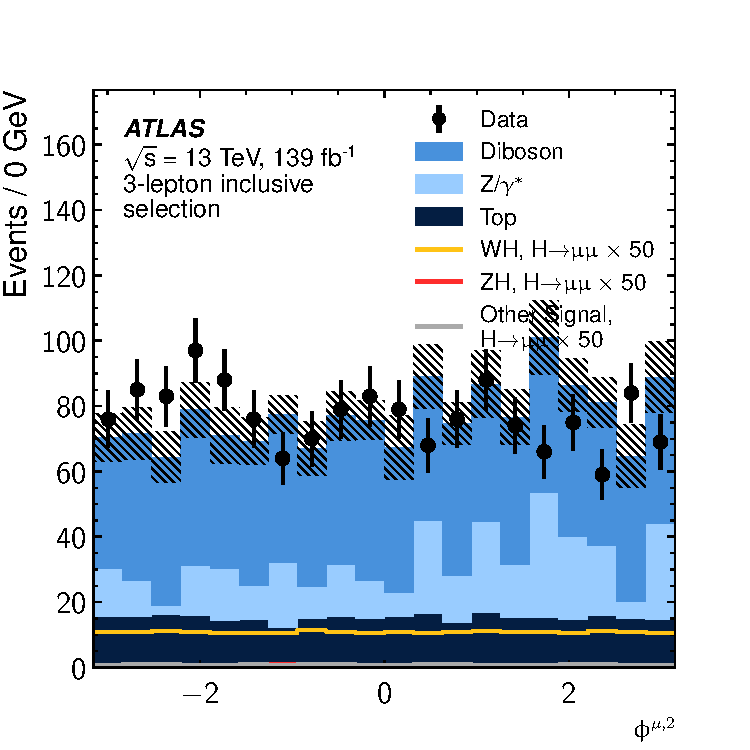
\includegraphics[width=0.4\textwidth]{figures/hmm/kinematics/histo-3lep-u2_phi.pdf}
  \caption{Kinematic plots showing $p_T$, $\eta$, and $\phi$ distributions for the H candidate muons from the 3-lepton selection.}
    \label{fig:hmmKineWhMuons}
\end{figure}

\clearpage
\begin{figure}[htpb]
  \centering
  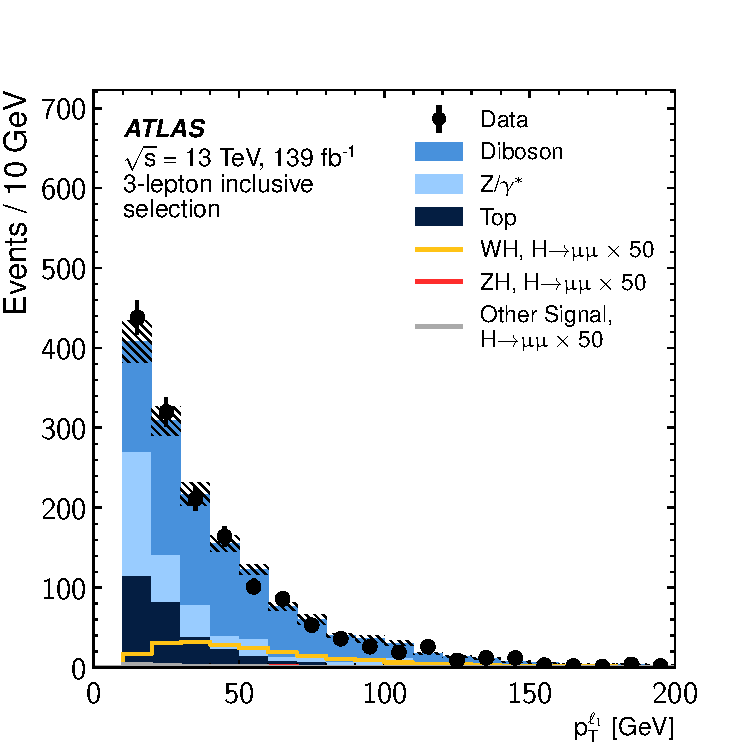
\includegraphics[width=0.4\textwidth]{figures/hmm/kinematics/histo-3lep-aux1_pt.pdf}\\
  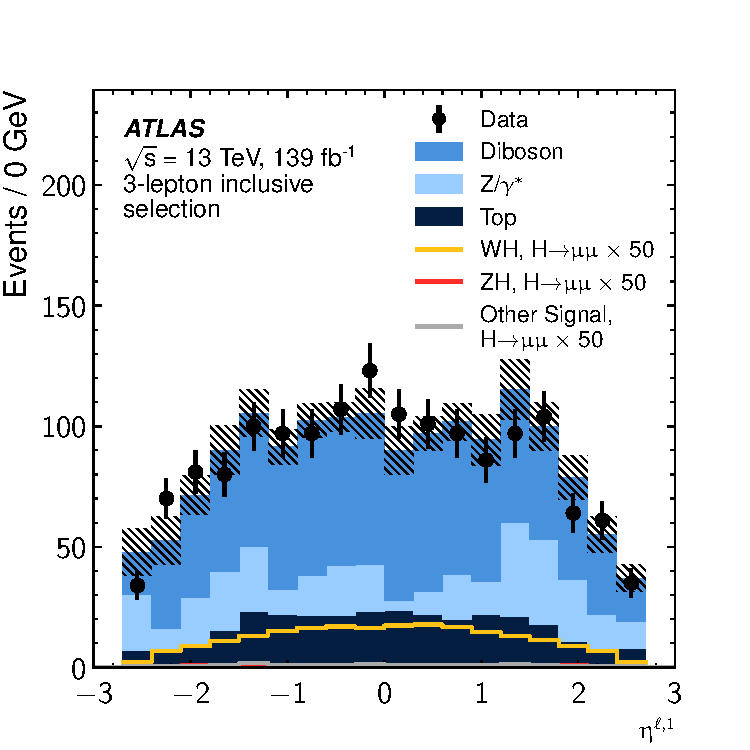
\includegraphics[width=0.4\textwidth]{figures/hmm/kinematics/histo-3lep-aux1_eta.pdf}\\
  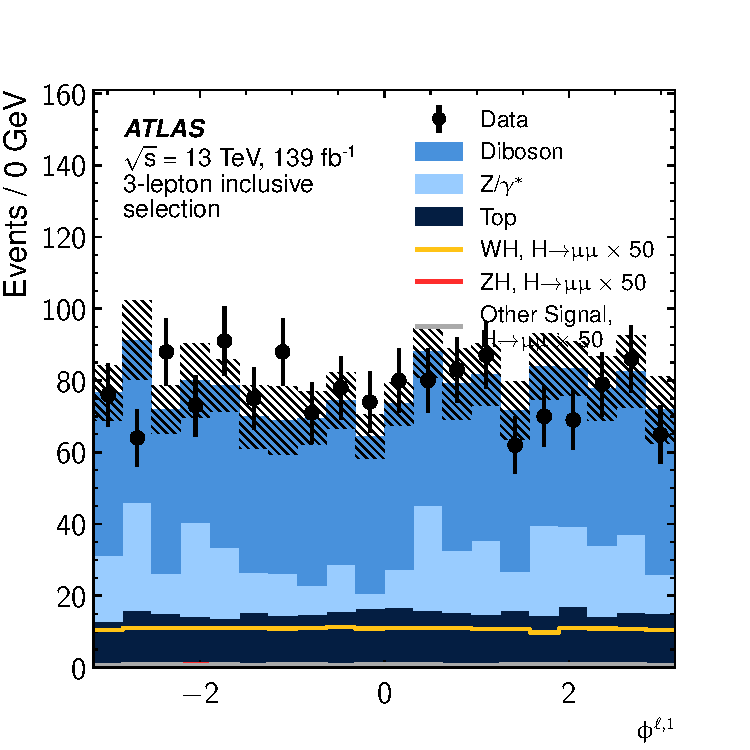
\includegraphics[width=0.4\textwidth]{figures/hmm/kinematics/histo-3lep-aux1_phi.pdf}\\
  \caption{Kinematic plots showing $p_T$, $\eta$, and $\phi$ distributions for the additional lepton/W candidate for the 3-lepton selection.}
    \label{fig:hmmKineWhLeps}
\end{figure}

\clearpage
\begin{figure}[htpb]
  \centering
  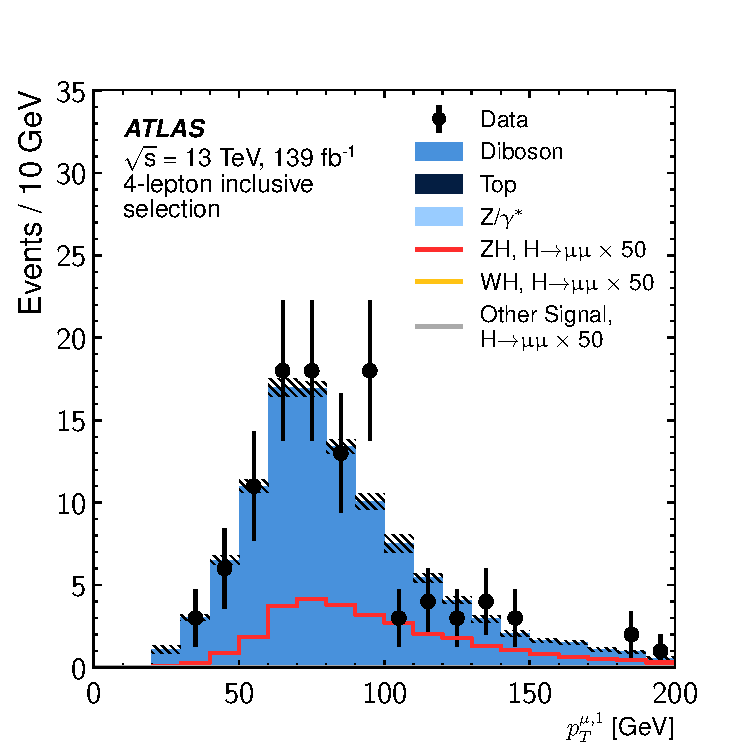
\includegraphics[width=0.4\textwidth]{figures/hmm/kinematics/histo-4lep-u1_pt.pdf}
  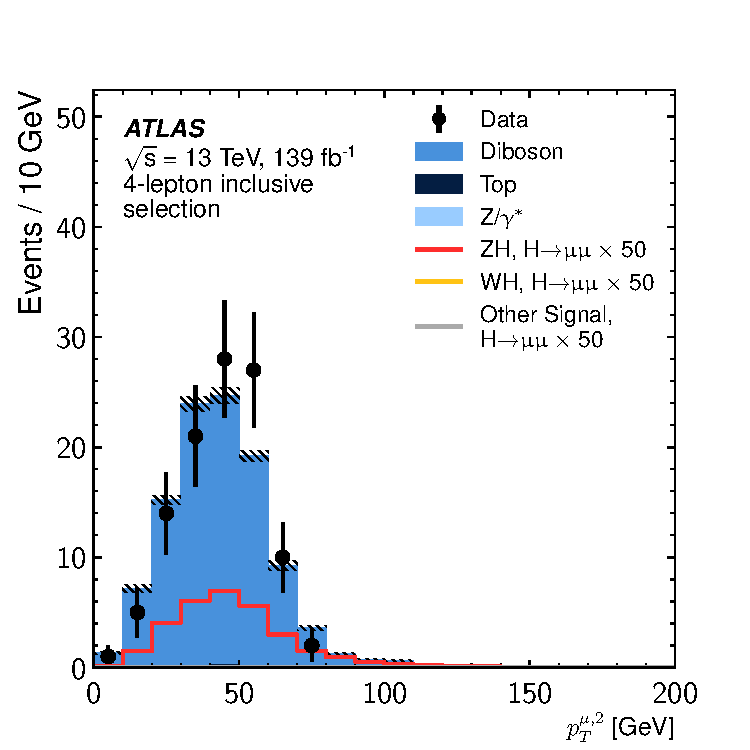
\includegraphics[width=0.4\textwidth]{figures/hmm/kinematics/histo-4lep-u2_pt.pdf}
  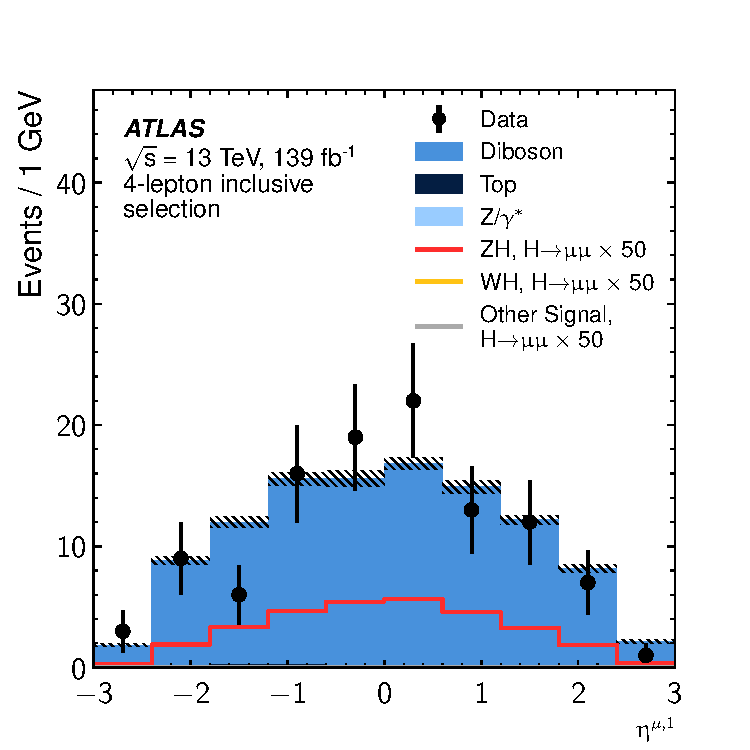
\includegraphics[width=0.4\textwidth]{figures/hmm/kinematics/histo-4lep-u1_eta.pdf}
  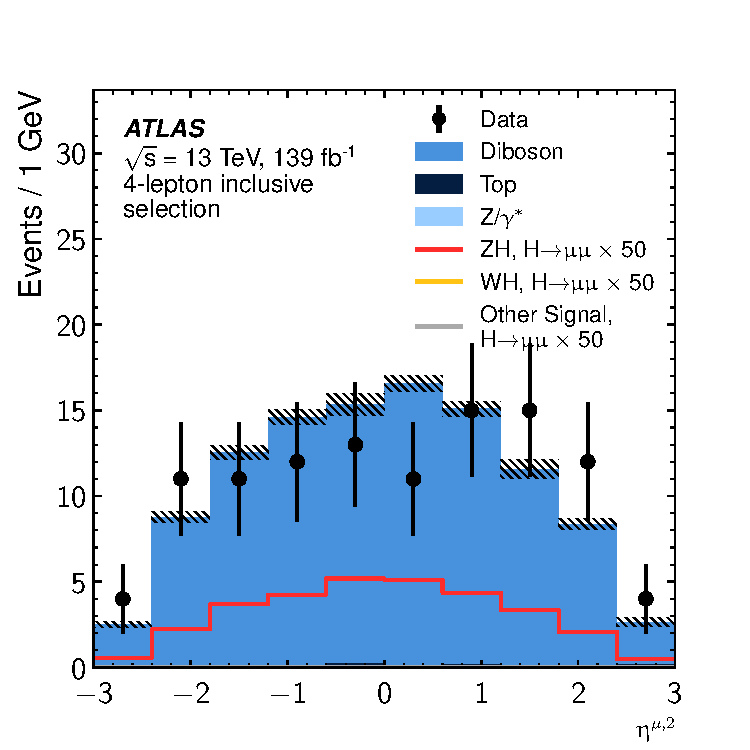
\includegraphics[width=0.4\textwidth]{figures/hmm/kinematics/histo-4lep-u2_eta.pdf}
  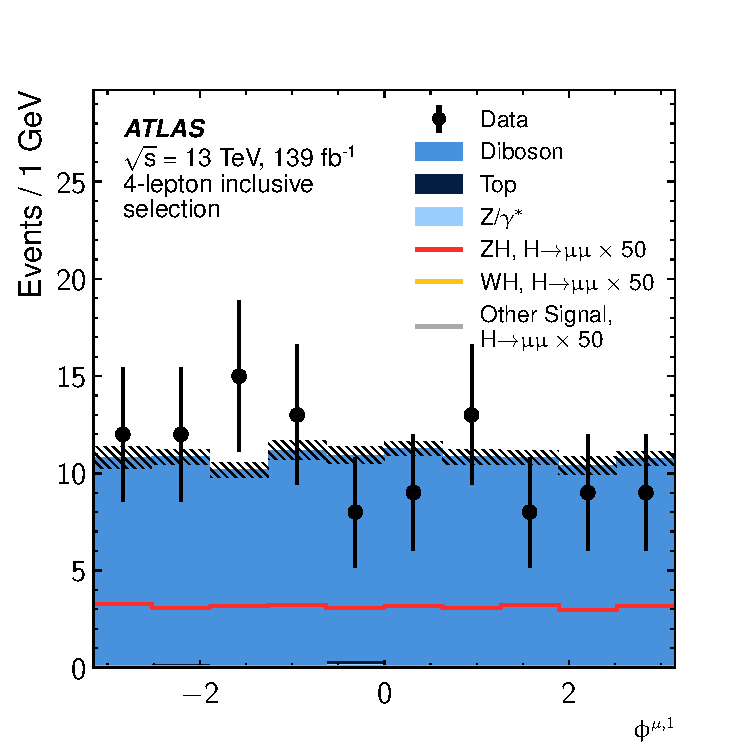
\includegraphics[width=0.4\textwidth]{figures/hmm/kinematics/histo-4lep-u1_phi.pdf}
  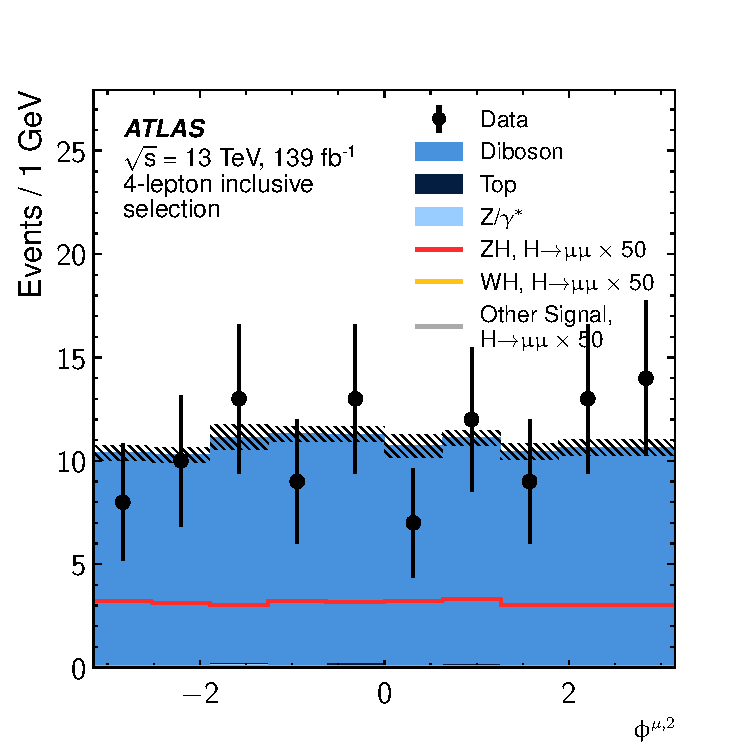
\includegraphics[width=0.4\textwidth]{figures/hmm/kinematics/histo-4lep-u2_phi.pdf}
  \caption{Kinematic plots showing $p_T$, $\eta$, and $\phi$ distributions for the H candidate muons from the 4-lepton selection.}
    \label{fig:hmmKineZhMuons}
\end{figure}

\clearpage
\begin{figure}[htpb]
  \centering
  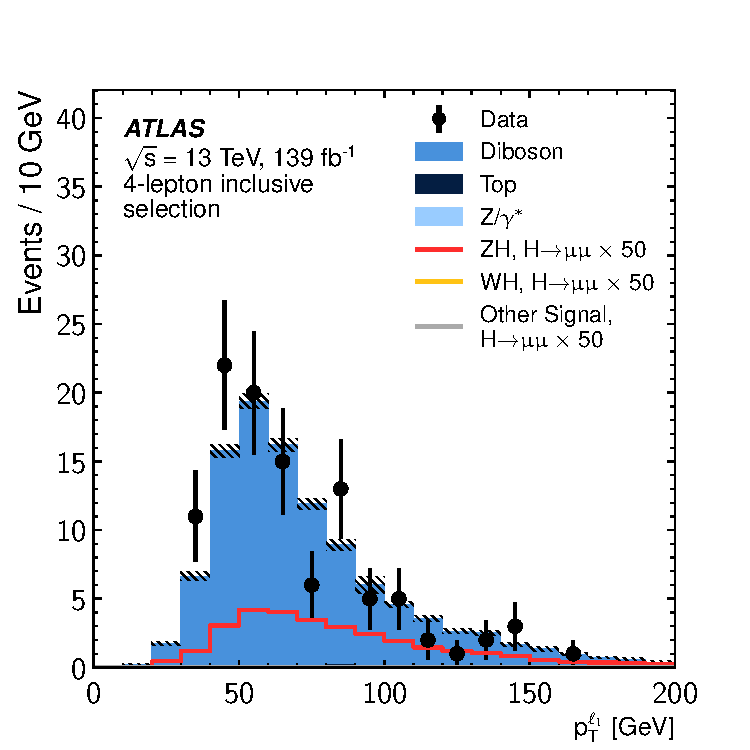
\includegraphics[width=0.4\textwidth]{figures/hmm/kinematics/histo-4lep-aux1_pt.pdf}
  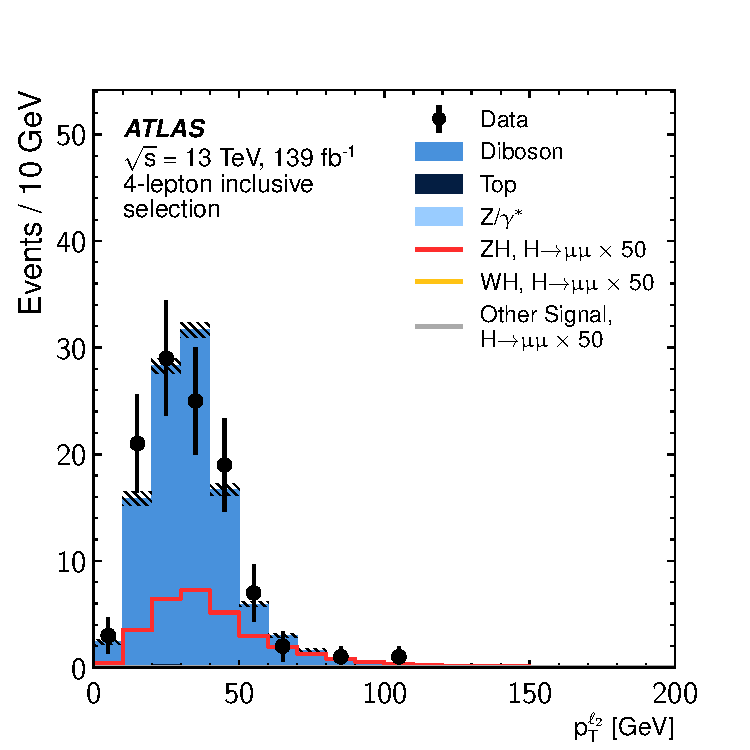
\includegraphics[width=0.4\textwidth]{figures/hmm/kinematics/histo-4lep-aux2_pt.pdf}
  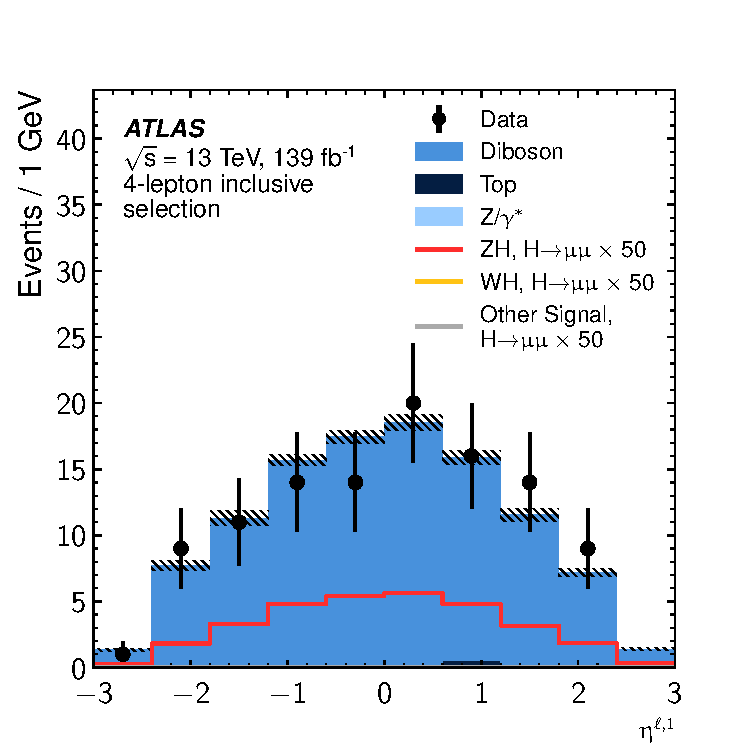
\includegraphics[width=0.4\textwidth]{figures/hmm/kinematics/histo-4lep-aux1_eta.pdf}
  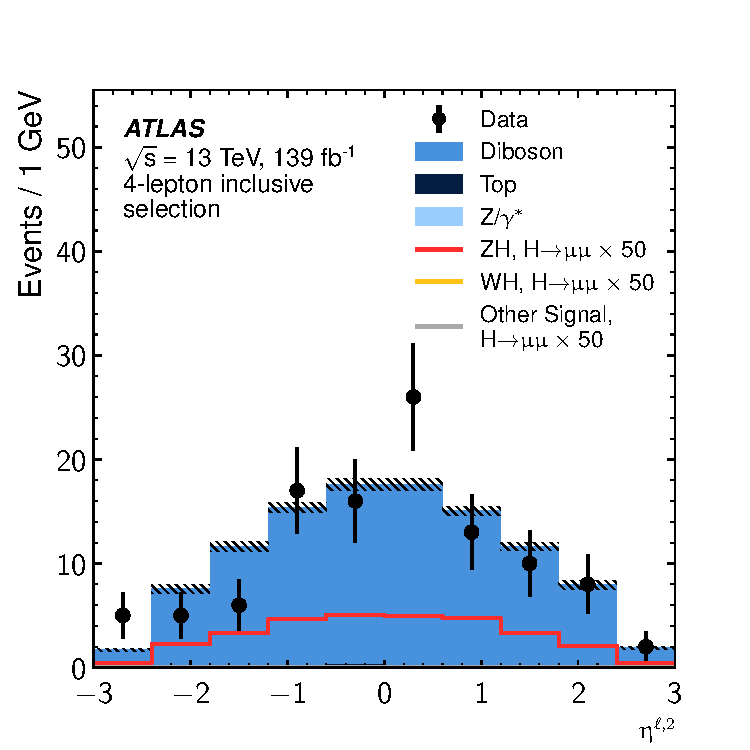
\includegraphics[width=0.4\textwidth]{figures/hmm/kinematics/histo-4lep-aux2_eta.pdf}
  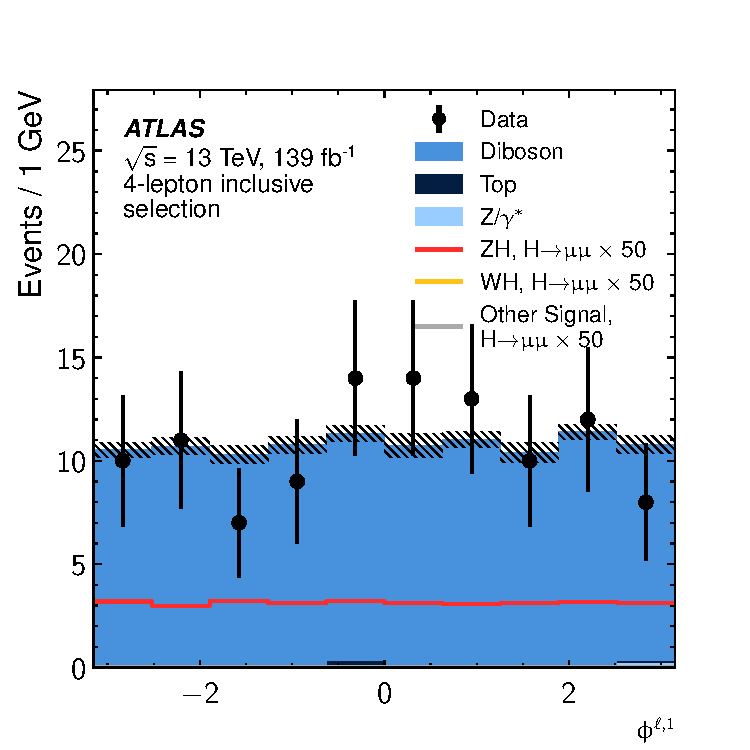
\includegraphics[width=0.4\textwidth]{figures/hmm/kinematics/histo-4lep-aux1_phi.pdf}
  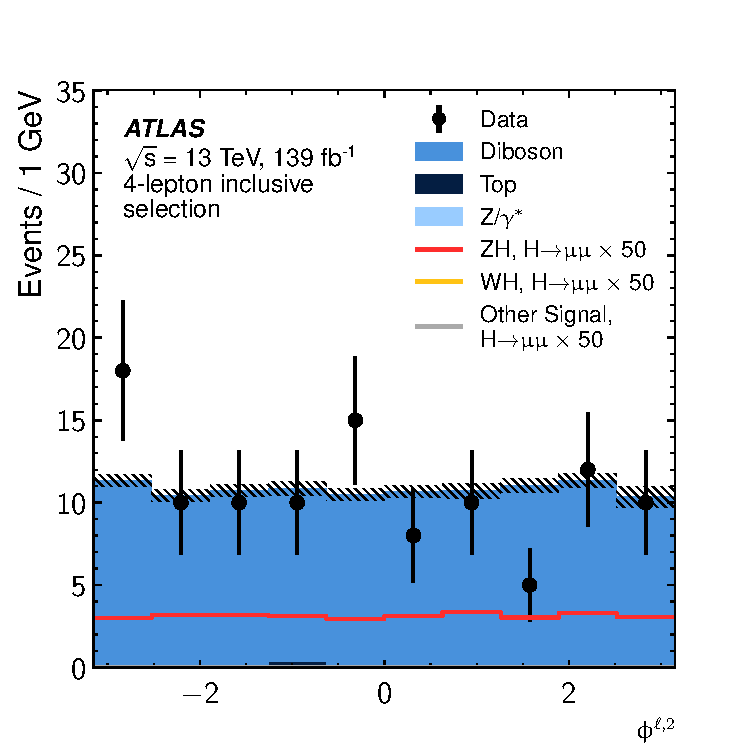
\includegraphics[width=0.4\textwidth]{figures/hmm/kinematics/histo-4lep-aux2_phi.pdf}
  \caption{Kinematic plots showing $p_T$, $\eta$, and $\phi$ distributions for the Z candidate leptons from the 4-lepton selection.}
    \label{fig:hmmKineZhLeps}
\end{figure}
\clearpage



\section{Multivariate Categorization}\label{sec:hmmBdt}

The events belonging to the inclusive 3-lepton and 4-lepton categories are further divided into exclusive sub-categories.
The definition of the exclusive categories is based on a multivariate discriminant that is a function of several kinematic variables.
The discriminant for classification is calculated using a \emph{boosted decision tree} (BDT).
This is a function of event kinematics that is defined to identify signal-like events from the larger set of background-like events.
It is derived based on the available information about signal and background kinematics from simulation.
This derivation, or \emph{training}, is performed by fitting the free parameters of the BDT to the available information.

\begin{figure}[h!]
\captionsetup[subfigure]{position=b}
\centering
\subfloat[][]{\label{fig:bdtTree}{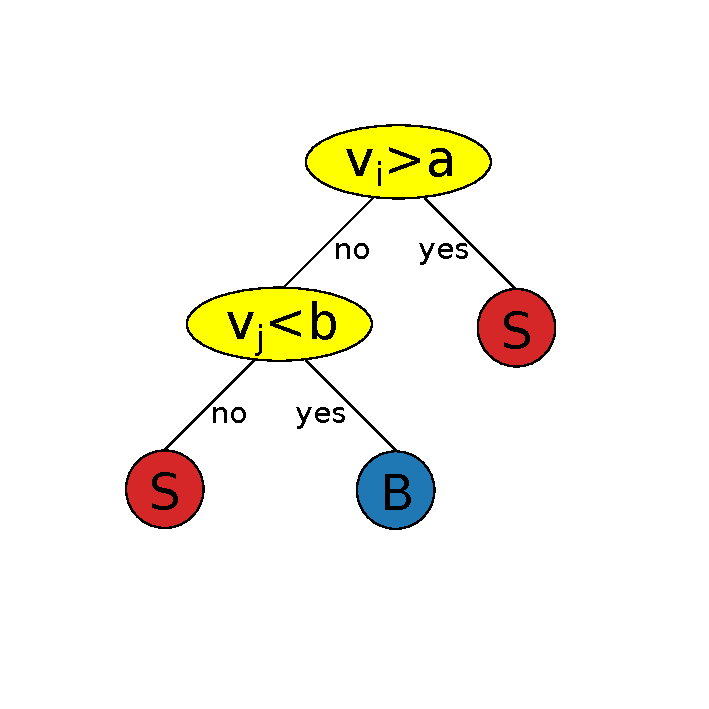
\includegraphics[scale=0.35]{figures/hmm/tree.pdf}}}
\subfloat[][]{{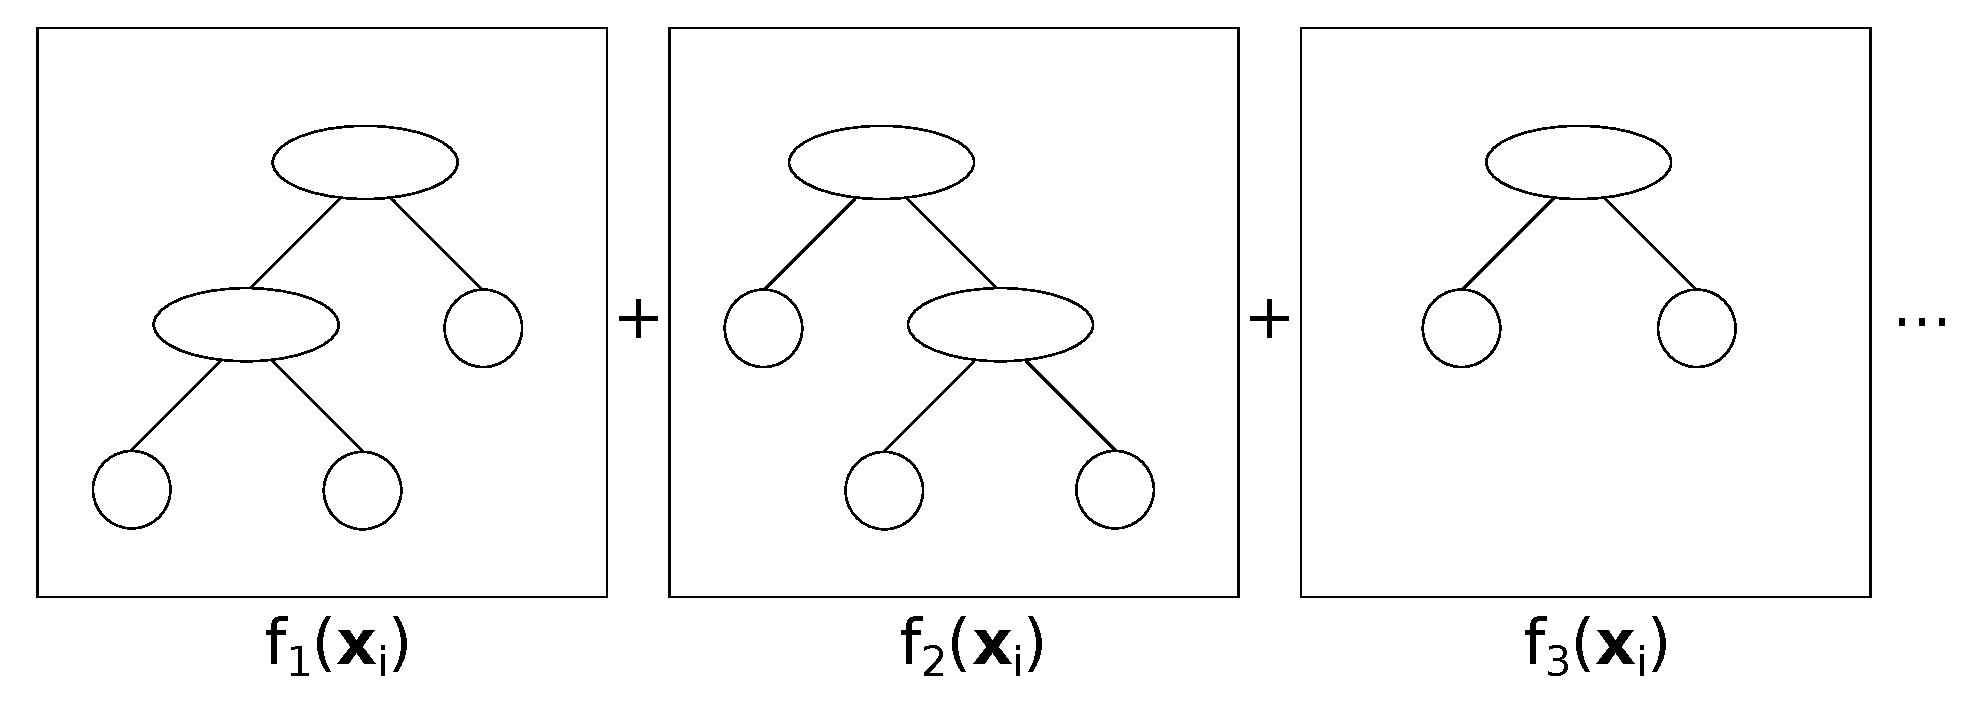
\includegraphics[scale=0.35]{figures/hmm/ensamble.pdf}}}
\caption{Figure (a) schematizes an individual decision tree, where in boolean splits based on the value of variables $v$ result in a categorization of signal or data as output. In a CART, the output is replaced by a continuous weight encoding ``signal-like'' versus ``background-like''. Figure (b) schematizes an ensemble of trees with different topologies, each defining an output function.}
\label{fig:}
\end{figure}

The information available for the training consists of datasets of $n$ entries and $m$ variables
The multi-dimensional entries $x_i$ $i\in[1,...,n]$ are labeled as either signal or background with $y_i$.
The elements of $x_i$ are variables $v_j$ $j\in[1,...,m]$.
The BDT is composed by of ensemble of decision trees.
A decision tree maps an entry of the dataset $x_i$ onto a discrete output space, such as a signal-vs-background likelihood.
Each node of the tree may represent a binary decision, or split, based on the variables of the entry.
Alternatively, the nodes with no children (leaves) may represent a decision, as illustrated in Figure \ref{fig:bdtTree}.
A generalization of a decision tree that assigns continuous weights to each leaf is a classification and regression tree (CART).
A tree can be \emph{trained} to map a set of input entries $x_i$ onto their corresponding labels $y_i$ by treating the distributions of input variables as PDFs and selecting splits (a, b, ...) that result in the highest output fidelity.
A single CART tends to struggle to represent the complexity of simulated physics datasets succinctly.
This performance can be augmented by an ensemble of CARTs labeled $k$, each with an output function $f_k(x_i)$ as illustrated in Figure \ref{fig:bdtTree}.
The output functions act as a \emph{model} of the provided dataset.
The sum of the CART output functions defines a new ensemble output function $f(x_i)=\hat{y}_i$, also called the discriminant score.

The training strategy is to develop an ensemble whose output functions accurately predict the corresponding label $y_i$ for unseen events.
This is quantified by a regularized loss function,
\begin{equation}\begin{split}\label{eqn:lossFunc}
    \mathcal{L}(\phi)=\sum_i l(\hat{y}_i,y_i),
\end{split}\end{equation} 
where $l$ measures the difference between $\hat{y}_i$ and $y_i$.
A process is defined to select trees, splits, and weights to minimize Equation \ref{eqn:lossFunc}.

The algorithm of \emph{boosting} is employed to minimize such loss functions by improving on the capability of a single CART.
It consists of iteratively expanding an ensemble of trees, with each addition addressing the mis-categorization of the previous ensemble.
One algorithm, \code{AdaBoost}, performs this task by iteratively reweighting poorly categorized entries to be more important to the following tree.
Another algorithm, \code{Gradient Boosting}, instead adds trees that are trained on the previous ensemble's poorly categorized entries.
Both of these algorithms played a role in the development of the analysis.
A descendent of \code{AdaBoost} and \code{Gradient Boosting} is \xgb, which introduces a modified loss function,
\begin{equation}\begin{split}\label{eqn:lossFuncXgb}
    \mathcal{L}(\phi)=\sum_i l(\hat{y}_i,y_i)+\sum_k \Omega(f_k).
\end{split}\end{equation} 
In Equation \ref{eqn:lossFuncXgb}, $\Omega$ is a measure of the complexity a tree.
The \xgb algorithm iteratively adds trees of diminishing weights, shrinking their importance by a constant factor.
It also introduces procedures to more quickly add and remove branches from trees while fitting the loss function.
These result in an accurate and reliable output function that can be trained quickly.
The \xgb algorithm was selected to construct the multivariate discriminant functions that are used in this analysis.
\cite{xgboost}

% Overtraining
It is a general goal to understand the underlying probability distributions that have produced a dataset, rather than of the dataset itself.
This applies to tasks such as training BDTs to discriminate signal from background, as well as fitting a functional form to data to model a background distribution. 
In both cases, the analytic model is interpreted as knowledge of these underlying distributions.
When solving an optimization problem such as those posed in Equations \ref{eqn:lossFunc} and \ref{eqn:lossFuncXgb}, the minimization algorithm has only the dataset at its disposal.
This can lead to \emph{over-training} or \emph{over-fitting}, where the optimization of the loss function tunes the discriminant to the features of a particular dataset rather than the features of the underlying distributions.
This problem tends to grow in step with the complexity of the model.
It is combatted, in part, by penalizing the optimization by the complexity of the model; the $\Omega$ function of Equation \ref{eqn:lossFuncXgb} is one such example.

Over-training may have two important and detrimental effects.
The first is to reduce the efficacy of the discriminant when applied to a new dataset.
Although this impacts the performance of the analysis, it does not necessarily invalidate the results by the introduction of bias.
The greater danger to the integrity of the analysis arises when the performance of the discriminant is inaccurately measured.
This second effect is illustrated in the following example.
Suppose a BDT is trained to identify signal events from a simulated dataset, and the same dataset is used to predict the number of signal events to expect in observed data.
A signal-rich category is defined based on the discriminant score for events.
In this case, simulated signal events tend to be over-represented in the category.
The BDT will identify simulated signal events with higher efficiency compared to signal in the data, leasing to an unconstrained uncertainty on the expected signal.
Unlike the first effect, this type of error invalidates the double use of the training simulation for further measurements.

\begin{figure}[h!]
\captionsetup[subfigure]{position=b}
\centering
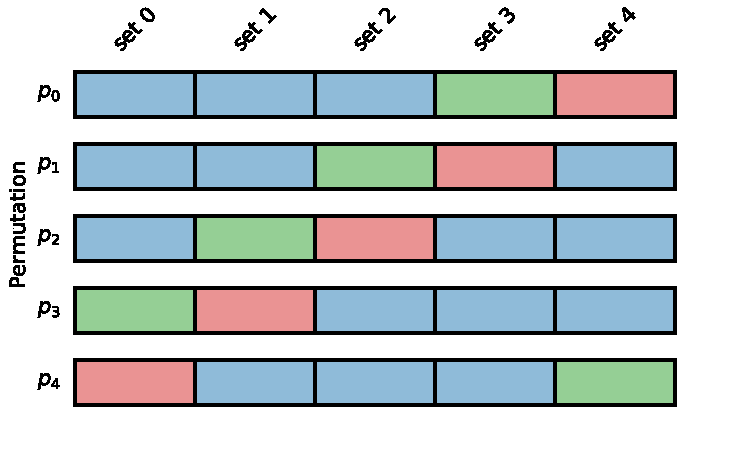
\includegraphics[width=0.75\textwidth]{figures/hmm/testTrainVal.pdf}
\caption{The top row, $p_0$, shows an schematization of a dataset divided into five subsets with $k$-fold split with $k=5$.
The blue boxes represent sets to be used for training, the green boxes for validation, the red boxes for testing.
Five permutations of these assignments, $p_i$, are shown for the same dataset.
In cross-validation, a separate MVA is fit to each permutation, such that each entry of the full dataset belongs to the testing set for a particular MVA.
}
\label{fig:testTrainVal}
\end{figure}

The problem of over-training is mitigated by introducing a $k$-fold split of the available simulated datasets into a number, $k>2$, of subsets of similar multiplicity.
One subset is labeled as the ``testing'' set, and another is labeled as a ``validation'' set.
The remaining subsets are combined as a ``training'' set.
This is illustrated in the top of Figure \ref{fig:testTrainVal}.
The BDT algorithm is deployed on the training set, and further predictions with respect to the simulation are performed with the testing set.
Since the testing set has not been exposed to the BDT during training, there is no direct risk of over-training of the discriminant scores in the testing set.
There remains the issue of selecting thresholds that define the signal-rich category to optimize, for example, the expected sensitivity.
This choice is subject to the same concerns about over-training as the selection of trees during the training phase. 
A third set, the validation set, is defined orthogonally to both the training and testing sets.
This set is used to study the convergence of the training process, check for over-training effects that may reduce sensitivity, and, most importantly, to choose the discriminant thresholds for further categorization.

The final consideration is to inefficiency that such a division of the simulation set entails.
Simulated events are computationally expensive to produce.
A \emph{cross-validation} scheme calls for the permutation of each of the $k$ subdivisions, such that each event appears once in a test set, available for further analysis.
This is shown in Figure \ref{fig:testTrainVal}.
A separate BDT is trained with the training set from each permutation.
This means that each event in the full dataset has one discriminant score from a BDT for which it is in the testing set, one for which it is in the validation set, and $k-2$ for which it was in the training set.
The scores from the BDT for which an event was in the testing and validation sets are the testing and validation scores, respectively.

\subsection{Configuration}
\label{sec:hmmBdtConfiguration}

% Training details
Separate classifiers are trained for 3-lepton and 4-lepton categories, but there are many similarities between these.
A 5-fold splitting of the available signal and background simulation is used.
It is important to note that the testing set remains blinded until all choices related to the categorization channels have been fixed.
The output of the BDT on the testing set is final, and it is essential to refrain from making choices related to the procedure based on the testing set.
A cyclic permutation of the 5-fold splitting is used, such that a separate BDT is trained for each fifth of the total simulation.

% Samples
Each BDT is trained using the simulated background, in which all background components are included.
The signal for the 4-lepton BDTs are the qqZH samples, while the signal for the 3-lepton BDTs are the W$^\pm$H samples.
The per-event weights arising from scale factors and reweighing, along with the event corresponding to the campaign luminosity, cross-section, are provided to the BDT.
Negatively weighted events are removed, and the signal and background weights are both normalized.
% Sample statistics
The numbers of available simulated events for training are shown in table \ref{tab:hmmSampleStatistics}.

\begin{table}[htbp]
 \caption{Numbers of simulated events available for training, both in the full simulation, and the 3/5 training sets statistics.}
 \begin{center}
\begin{tabular}{l r r r}\toprule
Simulation           & Total Events & Training Events \\
\midrule
4-lepton signal      & 20700        & 12508    \\
4-lepton background  & 88314        & 53081    \\
3-lepton signal      & 134936       & 80962    \\
3-lepton background  & 185286       & 111107   \\
\bottomrule\end{tabular} 
 \end{center}
\label{tab:hmmSampleStatistics}
\end{table}

% Training variables
The set of variables provided as input for the BDT was chosen from a broader set of candidate variables with physical motivations.
This set was reduced in the order of ascending \emph{feature importance}, defined as the number of times the variable is used for a decision node, weighted by the number of events categorized by the node during training.
The reduction continued until the performance of the BDT began to decline.
Different variables are defined based on the different final state topologies in the inclusive 4-lepton and 3-lepton categories.
The variables for each are listed in Table \ref{tab:hmmVarNames}.

\begin{table}[htp]
\caption{Variable names and definitions used training the 3-lepton ($3\ell$) and 4-lepton ($4\ell$) BDTs. The second column indicates the BDT in which the variable was used, based on the lepton category number.}
\begin{center}
\begin{tabular}{l c l l}
\toprule
Variable & Used for BDT & Definition \\
\midrule
  $m_T(E_T^\text{miss},l1)$ & $3\ell$ & Transverse mass of the W candidate lepton and $E_T^\text{miss}$  \\
  $\Delta_\phi(E_T^\text{miss},H)$ & $3\ell$ & $\phi$ between $E_T^\text{miss}$ and the H candidate \\
  $E_T^\text{miss}$ & $3\ell$ & Missing transverse momentum \\
  $p_T^{l1}$ & $3\ell$ & W candidate lepton $p_T$ \\
  $\Delta_\phi(l1,H)$ & $3\ell$ & $\Delta$ $\phi$ between H candidate and W candidate lepton \\
  $\Delta_\eta(l1,H)$ & $3\ell$ & $\Delta$ $\eta$ between H candidate and W candidate lepton \\
  $p_T^{j1}$ & $3\ell$ and $4\ell$ & $p_T$ of leading jet (if present) \\
  $N_\text{jets}$ & $3\ell$ and $4\ell$ & Number of jets \\
  $p_T^{j2}$ & $4\ell$ & $p_T$ of subleading jet (if present) \\
  $\Delta_\phi(l1,l2)$ & $4\ell$ & $\Delta$ $\phi$ between the leptons paired for the Z candidate \\
  $\Delta_\phi(Z,H)$ & $4\ell$ & $\Delta$ $\phi$ between H candidate and Z candidate \\
  $\Delta_\eta(Z,H)$ & $4\ell$ & $\Delta$ $\eta$ between H candidate and Z candidate \\
  $m_Z$ & $4\ell$ & Z candidate mass \\
\bottomrule
\end{tabular}
\label{tab:hmmVarNames}
\end{center}
\end{table}


\afterpage{
\begin{figure}[h!]
\captionsetup[subfigure]{position=b}
\centering
\subfloat[][]{{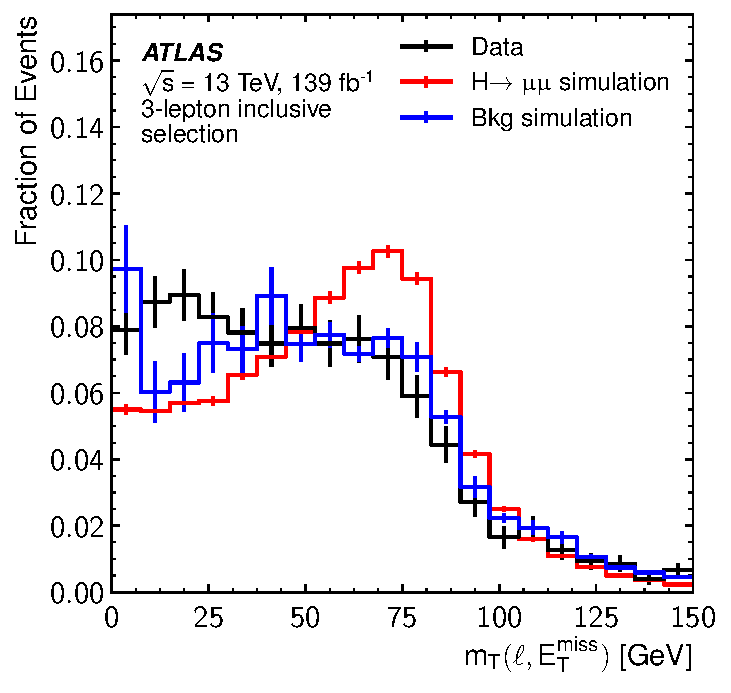
\includegraphics[width=0.35\textwidth]{figures/hmm/public/kine/kine-3lep-aux1_met_mt.pdf}}}
\subfloat[][]{{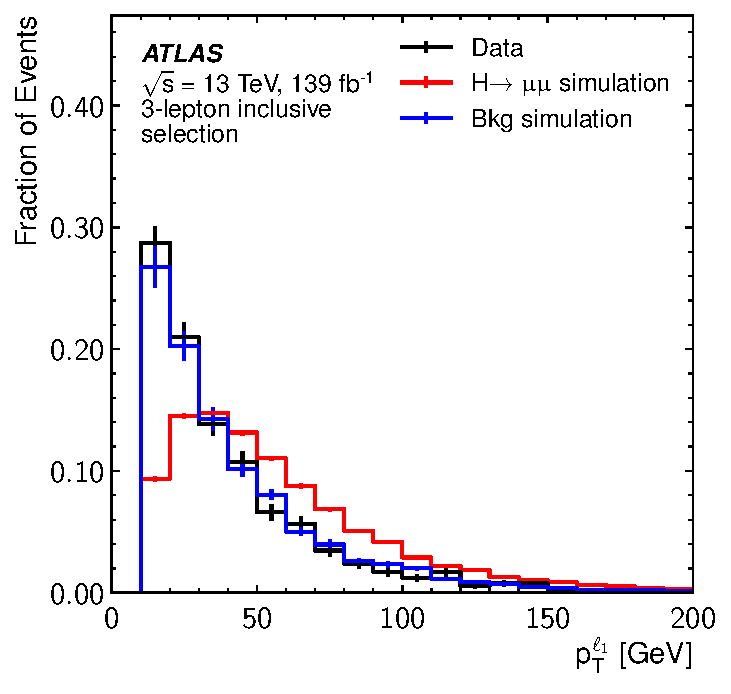
\includegraphics[width=0.35\textwidth]{figures/hmm/public/kine/kine-3lep-aux1_pt.pdf}}}
\subfloat[][]{{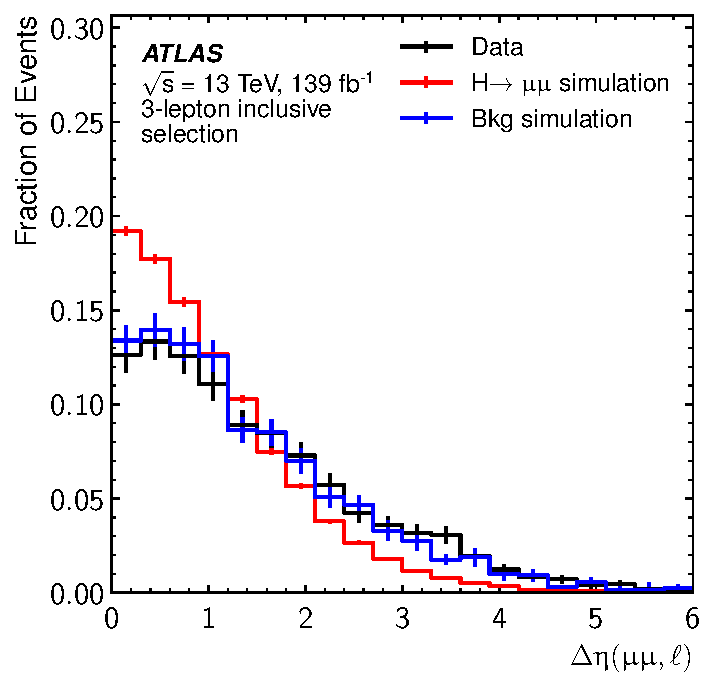
\includegraphics[width=0.35\textwidth]{figures/hmm/public/kine/kine-3lep-aux1_uu_delta_eta.pdf}}} \\
\subfloat[][]{{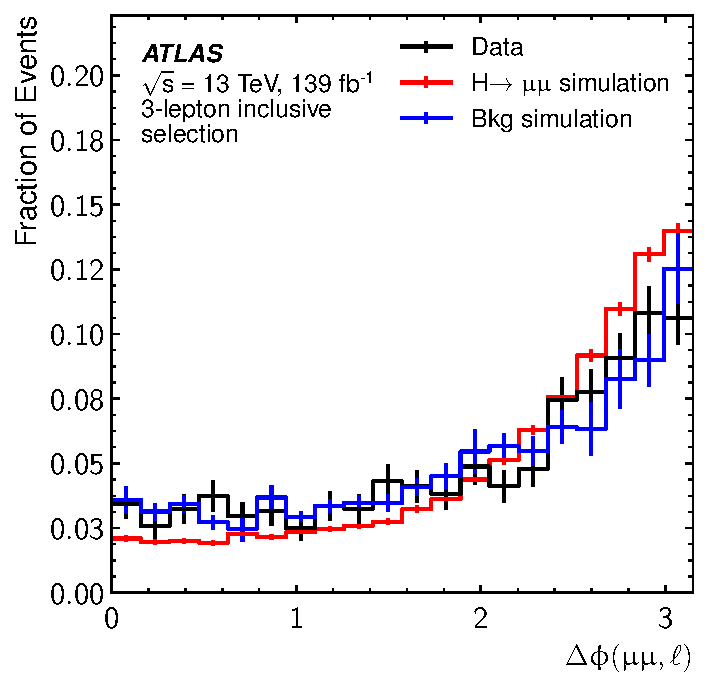
\includegraphics[width=0.35\textwidth]{figures/hmm/public/kine/kine-3lep-aux1_uu_delta_phi.pdf}}}
\subfloat[][]{{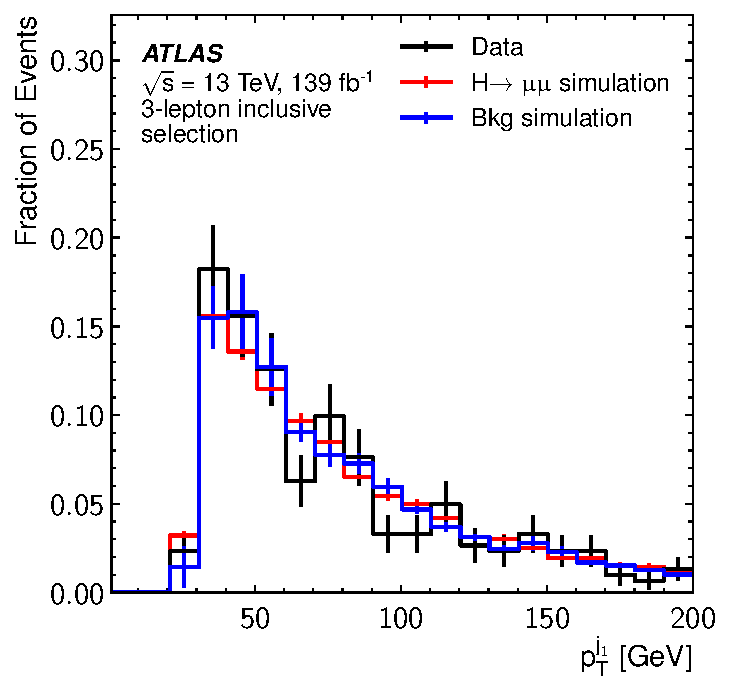
\includegraphics[width=0.35\textwidth]{figures/hmm/public/kine/kine-3lep-j1_pt.pdf}}}
\subfloat[][]{{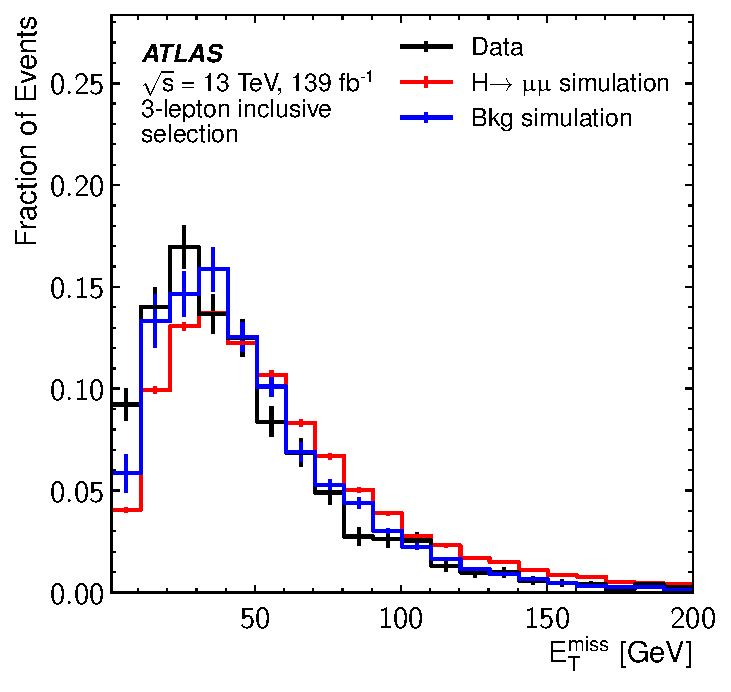
\includegraphics[width=0.35\textwidth]{figures/hmm/public/kine/kine-3lep-met_pt.pdf}}} \\
\subfloat[][]{{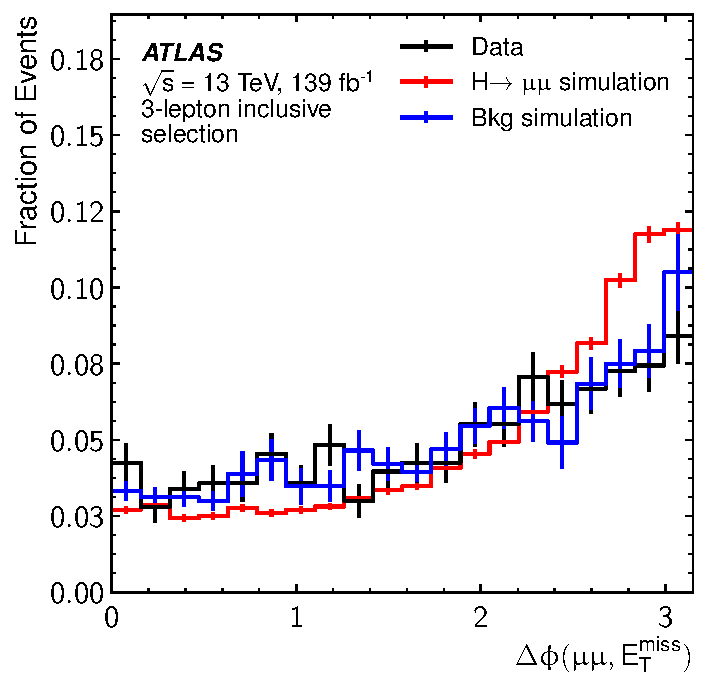
\includegraphics[width=0.35\textwidth]{figures/hmm/public/kine/kine-3lep-met_uu_delta_phi.pdf}}}
\subfloat[][]{{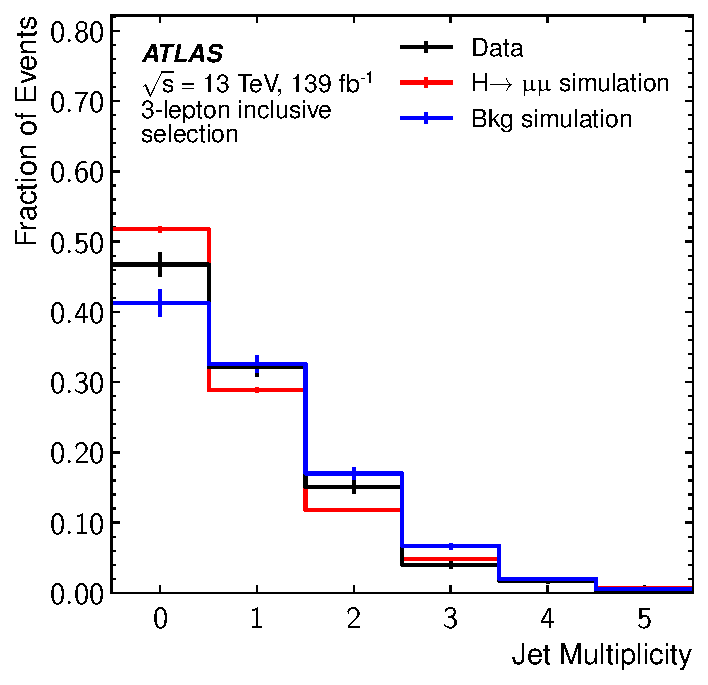
\includegraphics[width=0.35\textwidth]{figures/hmm/public/kine/kine-3lep-nJets.pdf}}}
\caption{Training variables provided as input for the for the 3-lepton classifier. The signal distribution shown in red is comprised of the simulated WH signal dataset, while the background distribution contains all background production modes shown in blue. Data distributions are included in black. Each distribution is normalized, and the error bars on each histogram are statistical only. }
\label{fig:hmm3lepVars}
\end{figure}
\clearpage
}

\afterpage{
\begin{figure}[h!]
\captionsetup[subfigure]{position=b}
\centering
\subfloat[][]{{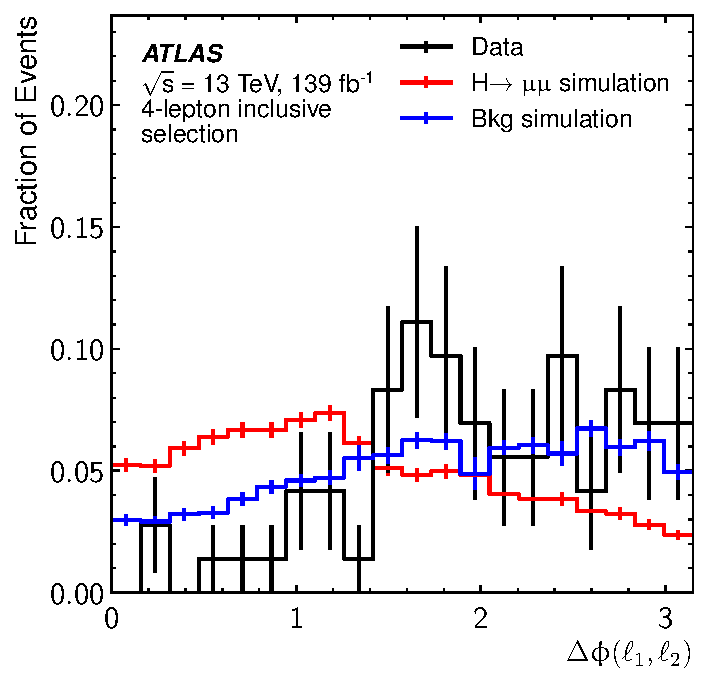
\includegraphics[width=0.35\textwidth]{figures/hmm/public/kine/kine-4lep-auxDilep_delta_phi.pdf}}}
\subfloat[][]{{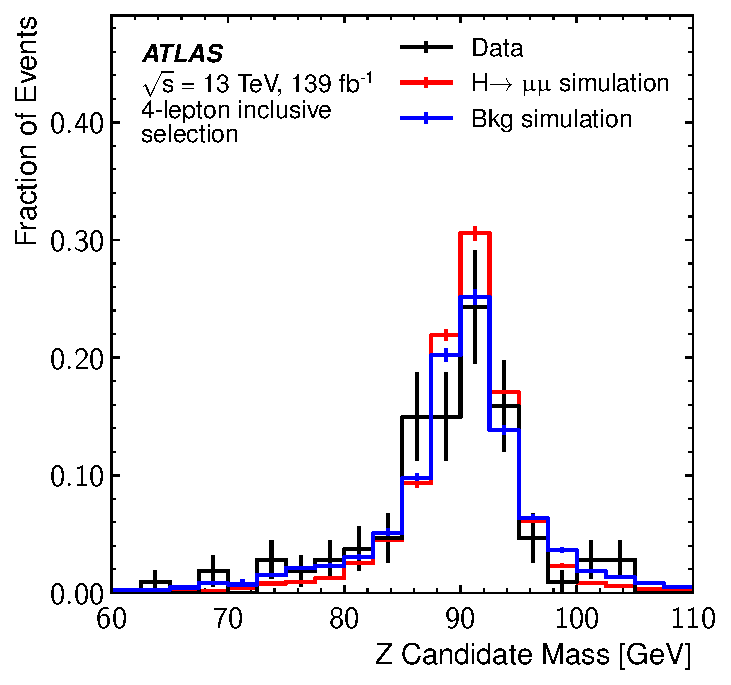
\includegraphics[width=0.35\textwidth]{figures/hmm/public/kine/kine-4lep-auxDilep_mass.pdf}}}
\subfloat[][]{{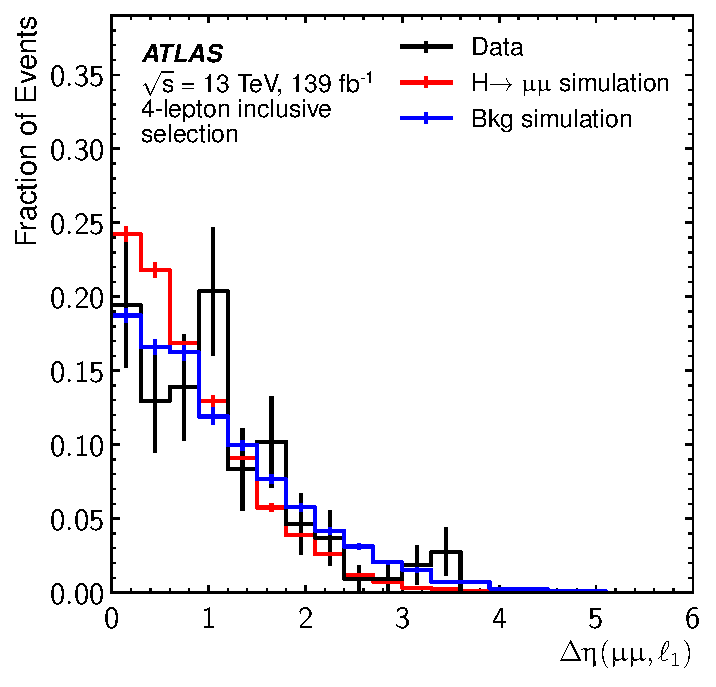
\includegraphics[width=0.35\textwidth]{figures/hmm/public/kine/kine-4lep-aux_uu_delta_eta.pdf}}} \\
\subfloat[][]{{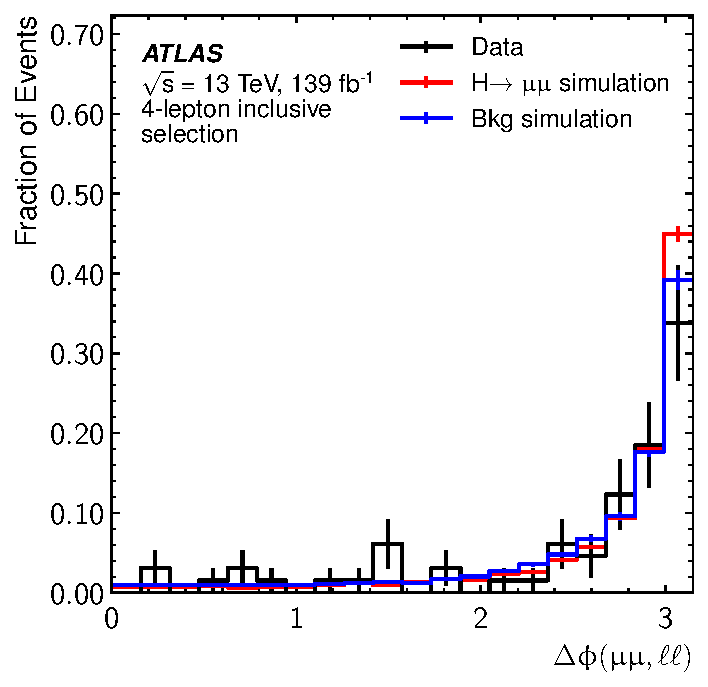
\includegraphics[width=0.35\textwidth]{figures/hmm/public/kine/kine-4lep-aux_uu_delta_phi.pdf}}}
\subfloat[][]{{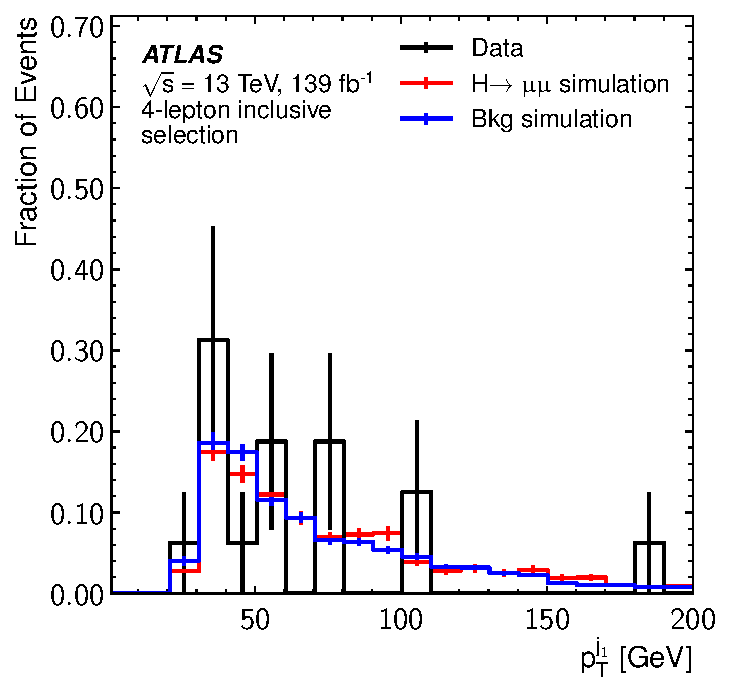
\includegraphics[width=0.35\textwidth]{figures/hmm/public/kine/kine-4lep-j1_pt.pdf}}}
\subfloat[][]{{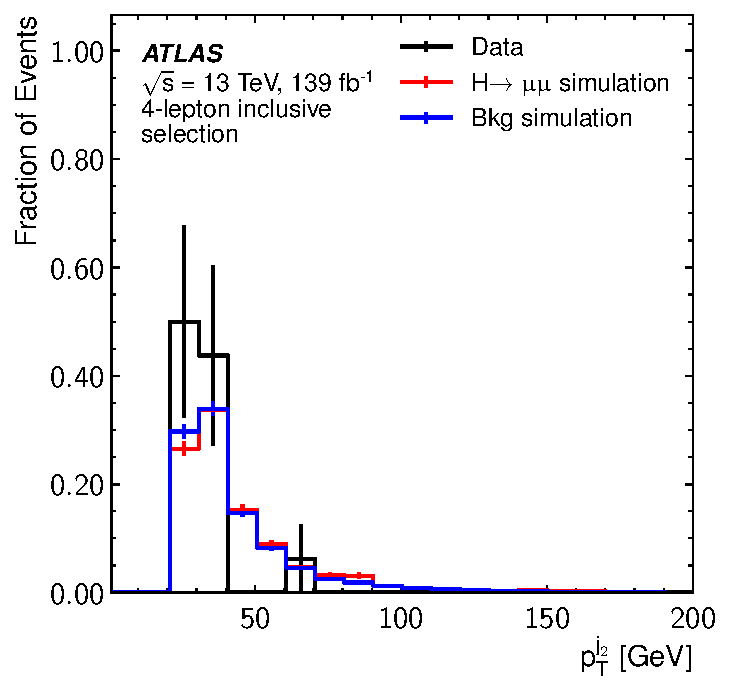
\includegraphics[width=0.35\textwidth]{figures/hmm/public/kine/kine-4lep-j2_pt.pdf}}} \\
\subfloat[][]{{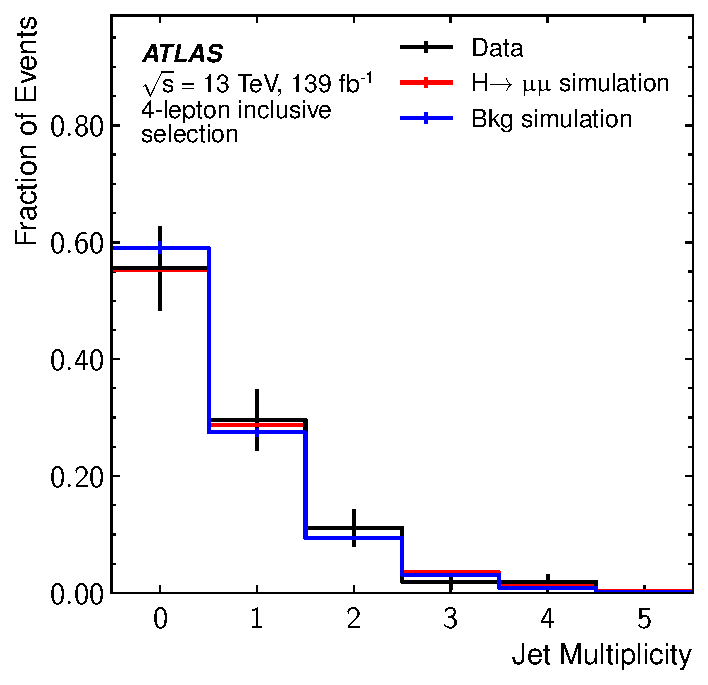
\includegraphics[width=0.35\textwidth]{figures/hmm/public/kine/kine-4lep-nJets.pdf}}}
\caption{Training variables provided as input for the for the 4-lepton classifier. The signal distribution shown in red is comprised of the simulated ZH signal dataset, while the background distribution contains all background production modes shown in blue. Data distributions are included in black. Each distribution is normalized, and the error bars on each histogram are statistical only. }
\label{fig:hmm4lepVars}
\end{figure}
\clearpage
}


%%%%%%%%%%%% Variable importance

% \begin{figure}[htpb]
%   \centering
%   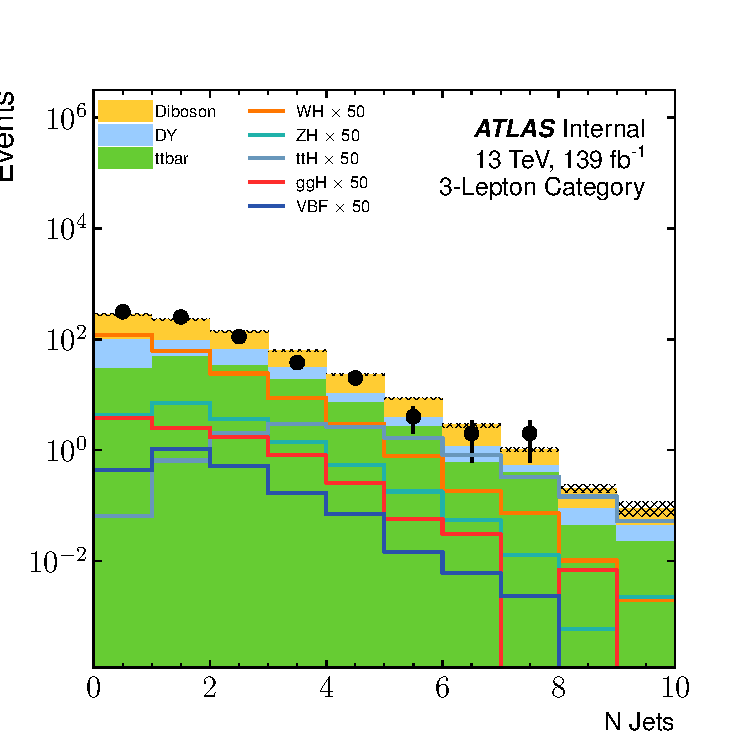
\includegraphics[height=0.48\textwidth]{figures/hmm/nJets/histo-3lep-nJets.pdf}
%   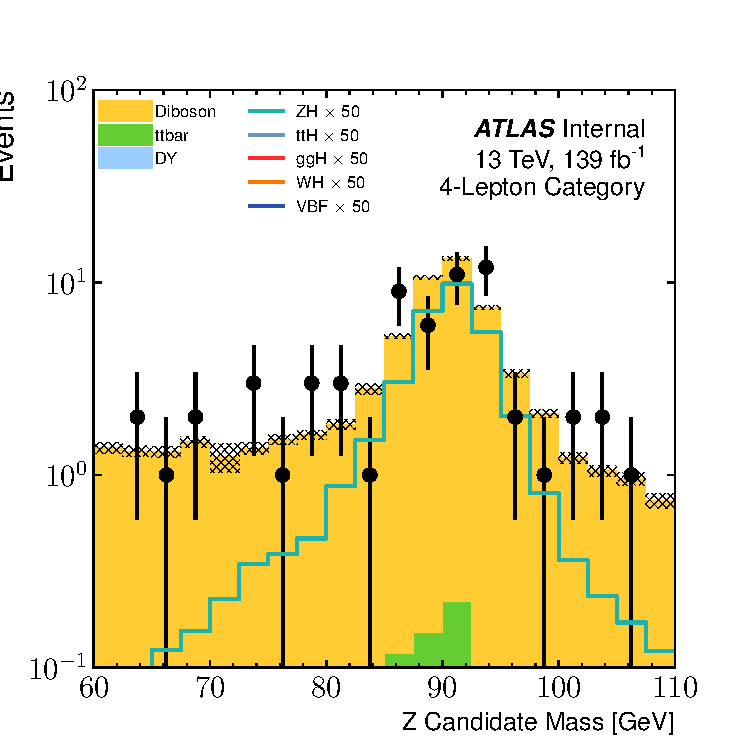
\includegraphics[height=0.48\textwidth]{figures/hmm/zCand/histo-4lep-auxDilep_mass.pdf}
%   \caption{Left: N Jets distribution for 3-lepton channel, right: Z candidate mass for 4-lepton channel. These are the highest ranked in feature importance for their category's respective BDT's.}
%     \label{fig:hmmImpVars}
% \end{figure}

The feature importances for each training case are listed in Tables \ref{tab:3lepVarImport} and \ref{tab:4lepVarImport}.
In the 4-lepton case, the most important variable is the mass of the \Z candidate, which helps identify the signal.
In the 3-lepton case, the most important variable is the number of jets, which helps especially to separate out top quark backgrounds.

% \begin{figure}[htpb]
%   \centering
%   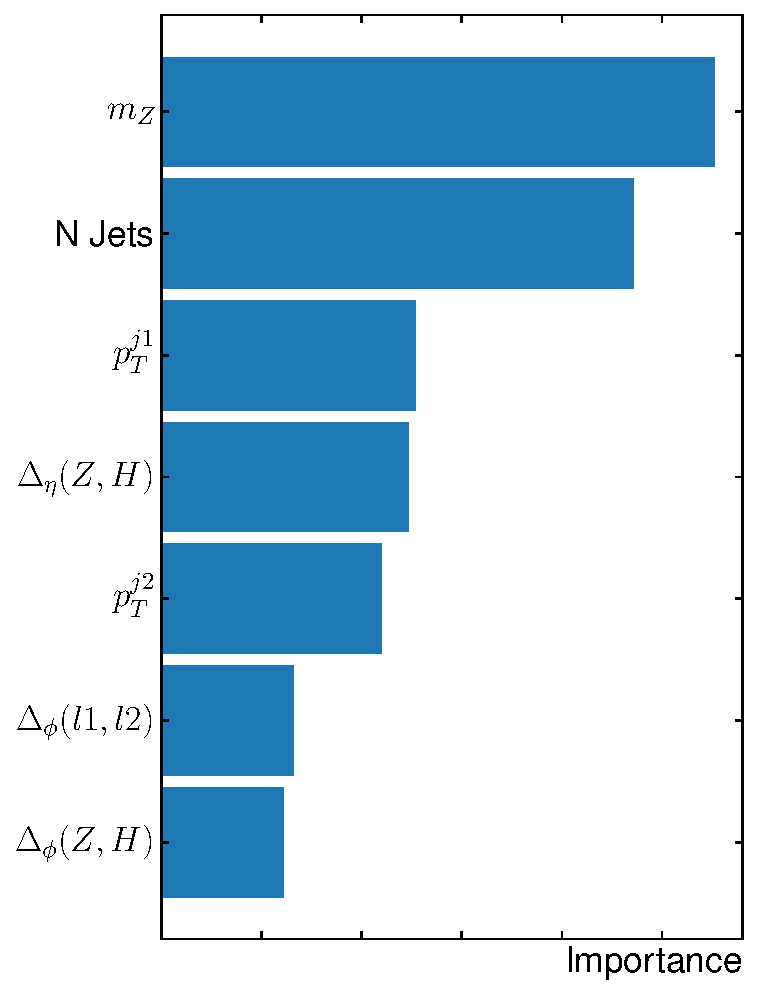
\includegraphics[height=8cm]{figures/hmm/bdtImportance/imp-4lep.pdf}
%   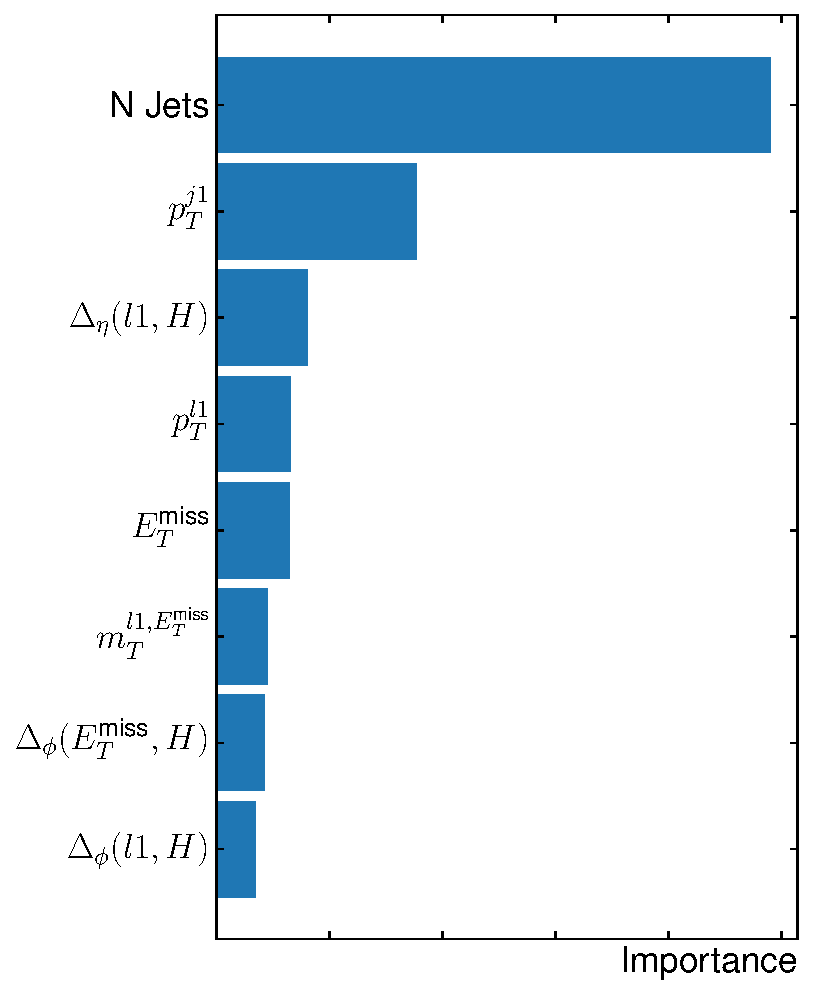
\includegraphics[height=8cm]{figures/hmm/bdtImportance/imp-3lep.pdf}
%   \caption{The 4-lepton (left) and 3-lepton (right) variables shown with their respective feature importance, averaged over the five BDTs trained for each cross-validation permutation. The importance of a variable is defined relative to the other variables.}
%     \label{fig:hmmVarImport}
% \end{figure}

\afterpage{
\begin{table}[htp]
\caption{Feature importance for the 3-lepton BDTs. The values shown are the feature importances normalized to the highest-importance variable. Values are given for individual BDTs along with a combined weight based on the sum across BDTs. The most important variable is the jet multiplicity.}
\begin{center}
\begin{tabular}{l ccccccc}
\toprule
Variable & BDT1 & BDT2 & BDT3 & BDT4 & Combined \\
\midrule
N Jets & 1.00 & 1.00 & 1.00 & 1.00 & 1.00 \\
$p_T^{j1}$ & 0.38 & 0.42 & 0.34 & 0.31 & 0.36 \\
$\Delta_\eta(l1,H)$ & 0.16 & 0.18 & 0.16 & 0.15 & 0.17 \\
$p_T^{l1}$ & 0.12 & 0.13 & 0.14 & 0.13 & 0.14 \\
$E_T^\text{miss}$  & 0.14 & 0.13 & 0.13 & 0.12 & 0.13 \\
$\Delta_\phi(E_T^\text{miss},H)$ & 0.09 & 0.08 & 0.10 & 0.10 & 0.09 \\
$m_T^{l1,E_T^\text{miss}}$ & 0.08 & 0.09 & 0.09 & 0.09 & 0.09 \\
$\Delta_\phi(l1,H)$ & 0.08 & 0.06 & 0.06 & 0.07 & 0.08 \\
\bottomrule
\end{tabular}
\label{tab:3lepVarImport}
\end{center}
\end{table}
%
\begin{table}[htp]
\caption{Feature importance for the 4-lepton BDTs, in the format of table \ref{tab:3lepVarImport}. The most important variable is the \Z candidate mass.}
\begin{center}
\begin{tabular}{l ccccccc}
\toprule
Variable & BDT1 & BDT2 & BDT3 & BDT4 & Combined \\
\midrule
$m_Z$ & 1.00 & 0.79 & 0.67 & 0.78 & 1.00 \\
N Jets & 0.99 & 1.00 & 1.00 & 1.00 & 0.89 \\
$p_T^{j1}$ & 0.78 & 0.44 & 0.19 & 0.25 & 0.60 \\
$\Delta_\eta(Z,H)$ & 0.45 & 0.39 & 0.37 & 0.51 & 0.55 \\
$p_T^{j2}$ & 0.12 & 0.41 & 0.49 & 0.58 & 0.31 \\
$\Delta_\phi(l1,l2)$ & 0.30 & 0.19 & 0.18 & 0.23 & 0.29 \\
$\Delta_\phi(Z,H)$ & 0.28 & 0.19 & 0.19 & 0.21 & 0.23 \\
\bottomrule
\end{tabular}
\label{tab:4lepVarImport}
\end{center}
\end{table}
\clearpage
}

The performance of a BDT is measured using the validation scores of the receiver operator curve (ROC).
The ROC is a parametric function of the BDT discriminant, plotted as the rate of correct signal categorizations (true positive rate) compared to the rate of false categorization of background as signal (false positive rate).
This is plotted in Figure \ref{fig:hmmBdtRoc} for a number of discriminant thresholds that define signal versus background.
A figure of merit used to evaluate the ROC is area-under-curve (AUC).
These show comparable performance for the BDTs of both categories and the impact of the relatively limited statistics of the 4-lepton sample.
As a cross check, the ROC curve for the training set is plotted along with the validation set. The agreement between these, within statistical uncertainty, does not indicate clear over-training effects.
The signal and background samples shown in the ROC plots correspond to the same samples used for the training; only WH and ZH signals are used in the definition of the ROC.

\begin{figure}[htpb]
  \centering
  \includegraphics[width=0.48\textwidth]{figures/hmm/bdtHist/roc-4lep-ZH-AllBackground-0-depth2-nEst80tag-new-AllBackground.pdf}
  \includegraphics[width=0.48\textwidth]{figures/hmm/bdtHist/roc-3lep-WH-AllBackground-0-depth2-nEst50tag-new-AllBackground.pdf}
  \caption{4 lepton (left) and 3 lepton (right) ROC curves for representative BDT's. Shown in black is the curve for the training set, while red shows the curve for the validation set (labeled test set). Error bars are statistical uncertainties due to the size of the training and validation datasets. The AUC is labeled on each plot.}
    \label{fig:hmmBdtRoc}
\end{figure}

% Figure \ref{fig:hmmBdtScoreLin} shows distributions of the BDT discriminant for different categories of signal and background, scaled the samples cross-section and luminosity.
% The signal/background separation is more apparent in this plot than in those normalized to the physical expectation.


% \begin{figure}[htpb]
%   \centering
%   \includegraphics[width=0.48\textwidth]{figures/hmm/bdtHist/bar20-4lep-ZH-AllBackground-0-depth2-nEst80tag-new-AllBackground.pdf}
%   \includegraphics[width=0.48\textwidth]{figures/hmm/bdtHist/bar20-3lep-WH-AllBackground-0-depth2-nEst50tag-new-AllBackground.pdf}
%   \caption{4 lepton (left) and 3 lepton (right) distributions of the BDT discriminant, where the signal and background samples share a normalization. The signal distribution is that of the sample used for training, not the full signal MC sample.}
%     \label{fig:hmmBdtScoreLin}
% \end{figure}

Figure \ref{fig:hmmBdtScore} shows the BDT discriminant calculated in different categories and scaled by the samples cross-section and luminosity.
The signal and background composition is more apparent in these plots: primarily, the target signal production mechanism is separated from other signals.
The top backgrounds are particularly well separated owing in part to the high statistics available for these samples in the training sets.

% {\color{red} This paragraph section is slightly redundant. Merge into next section?}
% Exclusive categories are defined based on discriminant cuts that produce varying levels of signal purity.
% The category ``4-lepton high-purity'' is defined in the 4-lepton selection by requiring 4-lepton BDT score greater than 0.12. 
% Two categories are defined from the 3-lepton selection: ``3-lepton high-purity'' and ``3-lepton middle-purity''. 
% The former is selected by requiring 3-lepton BDT score greater than 0.7,
% and the latter is selected by requiring 3-lepton BDT score less than 0.7
% but greater than 0.1.
% The events failing VH categorization are still considered in the inclusive categories.
 
\begin{figure}[htpb]
  \centering
  \includegraphics[width=0.48\textwidth]{figures/hmm/public/bdt/histo-4lep-bdtScore.pdf}
  \includegraphics[width=0.48\textwidth]{figures/hmm/public/bdt/histo-3lep-bdtScore.pdf}
  \caption{4-lepton (left) and 3-lepton (right) distributions of the BDT discriminant, using the final test scores. The simulated background is shown in shaded grey, while the signal distributions are drawn as lines in red for ZH and orange for WH. The remaining non-VH production mechanisms (ggF, VBF, and ttH) are combined and plotted as a dark grey line. All the signal histograms have been scaled by a factor of 50 to enhance visibility.\\
  It is observed that the score separates the signal to the left and background to the right. Of similar importance is that it specifically isolates the VH signal of interest and not the other signal productions. For 4-lepton this is the ZH signal and for 3-lepton this is the WH signal. Vertical dotted lines indicate the values that delineate which events belong in which final categories. The full dataset is included as well, which is used to fix the normalization of the background. \\
  The 3-lepton discriminant separates signal from background to a higher degree than does the 4-lepton discriminant. This is due in part to the stricter 4-lepton event selection, which can remove many more ``easily'' separable background events. The remaining events are more similar, topologically, to the ZH signal.}
    \label{fig:hmmBdtScore}
\end{figure}

\subsection{Categorization}

The event selection results in two inclusive categories distinguished by lepton number: the 4-lepton and 3-lepton categories.
These selections are further divided into \emph{exclusive} categories based on the relative purity of the signal.
This subsequent division is based on the BDT discriminant scores for each event.
The 4-lepton category is divided once into low-purity and high-purity categories.
The 3-lepton category, with a greater event multiplicity, is divided into low-, medium-, and high-purity categories.

Each event belongs to both a validation dataset and a testing dataset, each of which has an associated discriminant score.
The validation scores are considered when selecting the score thresholds delineating categories.
The testing scores are used for the final hypothesis test and limit setting.
An optimization scan over various thresholds of the expected significance determines the threshold values.
The thresholds are selected in order to produce the highest expected significance, based on the validation scores.
These thresholds are specified in Table \ref{tab:hmmBdtCuts}.

\begin{table}[htp]
\caption{Category definitions based on the ranges of the discriminant value $O$. The output of the BDT is scaled such that $O\in[0,1]$, with higher numbers corresponding to VH-like events.}
\begin{center}
\begin{tabular}{c c c l l l}
\toprule
Inclusive Category & Exclusive Category & Criteria \\
\midrule
\multirow{2}{*}{4-Lepton} & High-purity & $O\ge0.12$ \\
                          & Low-purity & $O<0.12$ \\
\midrule
\multirow{3}{*}{3-Lepton} & High-purity & $O\ge0.72$ \\
                          & Middle-purity & $0.10\ge O<0.72$ \\
                          & Low-purity & $O<0.10$ \\
\bottomrule
\end{tabular}
\label{tab:hmmBdtCuts}
\end{center}
\end{table}

To first choose the thresholds using the testing set and then perform a hypothesis test in categories defined by that threshold would lead to a misleading signal and background expectation in those categories.
The choice of threshold would be biased to the statistical fluctuations in the test dataset.
This results in categories biased to contain more simulated signal events and fewer simulated background events than would be expected in the data.
Since the analysis of the data includes the signal model based on simulation, such a method is unacceptable.

\begin{figure}[htpb]
  \centering
  \includegraphics[width=0.45\textwidth]{figures/hmm/public/postCut/histo-4lep0-muu.pdf} \\
  \includegraphics[width=0.45\textwidth]{figures/hmm/public/postCut/histo-3lep0-muu.pdf} 
  \includegraphics[width=0.45\textwidth]{figures/hmm/public/postCut/histo-3lep1-muu.pdf} 
\caption{Distributions of \muu in the 4-lepton (top) and 3-lepton (bottom) selections after categorization based on a cut on the BDT discriminant score.}
    \label{fig:hmmPostcutMassHists}
\end{figure}
\clearpage

The high and middle-purity categories are considered for further analysis.
The low-purity events, containing few expected signal events, are only analyzed in the inclusive categories defined prior to BDT cut.
The distributions of \muu are shown in Figures \ref{fig:hmmPrecutMassHists} and \ref{fig:hmmPostcutMassHists}.
The former shows the inclusive distribution before further categorization with the BDT discriminant.
The latter shows the distributions in the categories defined in Table \ref{tab:hmmBdtCuts}.
The motivation to use the discriminant becomes apparent in these plots when compared to Figure \ref{fig:hmmPrecutMassHists}.
In both the 4-lepton and 3-lepton high-purity categories, Drell-Yan production has been virtually removed.
The background remaining is primarily from diboson sources.
The signal selection purity is also evident in the high-purity categories: these produce homogeneous selections of events from ZH or WH productions, depending on their target.


\section{Background Modeling}\label{sec:hmmBkg}

The results of this analysis are based on a comparison between signal and background hypotheses.
The simulated background distributions provide a powerful tool to understand the composition and kinematics of the backgrounds in each category.  
These also provide a possible definition for a background hypothesis, but this definition imports many theoretical assumptions.
Instead, an analytic background is developed from the data by fitting a functional form to the observation.

The Figures \ref{fig:hmmPrecutMassHists} and \ref{fig:hmmPostcutMassHists} show the \muu shapes of the simulated background distributions in the pre-cut and post-cut categories respectively.
In all cases, the background is characterized by a steeply falling \muu distribution with substantial contributions from \Z processes.
This motivates the inclusion of a Breit-Wigner shape in the functional form with the parameters of the \Z boson.
It is also important for the form to be flexible enough to describe the underlying background distribution without being flexible enough to describe the observed dataset's statistical fluctuations.
This motivates the inclusion of an exponential term that introduces only one flexible parameter.
The function chosen is defined in Equation \ref{eqn:hmmBkgFunc}. 
\begin{equation}\begin{split}\label{eqn:hmmBkgFunc}
    f_\text{B}(\muu) = (1-a)\times [f_{\text{BW},Z}\otimes\text{Gaus}()]+a\times\exp{b\times\frac{\muu-110\text{ GeV}}{160\text{ GeV}}}
\end{split}\end{equation} 
Here, \muu is the invariant-mass of the Higgs candidate dimuon, in GeV.
The Breit-Wigner function, $f_{\text{BW},Z}$ (defined in Equation \ref{eqn:breitWigner}), uses the \Z mass $m_\text{BW}=91.2$~GeV and width $\Gamma_\text{BW}=2.49$~GeV.
It is convolved with a Gaussian, the product of which is a Voigtian shape.
The Gaussian helps describe detector resolution effects and is centered at \muu with a width 2~GeV.
Two parameters are left to be determined by their agreement to the data.
The first, $a\in[0,1]$, represents the fraction of the background made of Breit-Wigner compared to the exponential term.
The second, $b$, determines the decent of the exponential term.
Equation \ref{eqn:hmmBkgFunc} is used to define a probability density function (PDF) over \mll from which observed events may have been sampled. 
When it is used to model the dataset, the PDF is normalized to the number of events in the dataset by a coefficient.
Since this coefficient is a function of $a$ and $b$, and it does not impact the shape of the distribution, it is suppressed.

The procedure to determine the free parameters is referred to as \emph{fitting} the functional form to the observed data.
The \code{minuit} algorithm \cite{roofit} is used to adjust the free parameters in order to maximize the likelihood that the observed data could be generated by the PDF.
This is performed in each category, and the resulting parameters are given in Table \ref{tab:hmmBkgFitParams}.

\begin{table}[htp]
\caption{Values of $a$ and $b$ fitted to the data in pre-cut (top) and post-cut (bottom) categories. Uncertainties are the statistical constraint of the fit. In the case of the lower multiplicity 4-lepton categories, the constraints on the parameters are $\sim60\%$ correlated, and one of them could be fixed. However this results in a biased estimate of the signal contribution, described in the following section.}
\begin{center}
\begin{tabular}{l r r r r r r}
\toprule
Category & $a$ & $b$ \\
\midrule
3-lepton & 0.96$\pm$0.13 & -5.08$\pm$0.61 \\
4-lepton & 1.00$\pm$1.00 & -5.75$\pm$1.17 \\
\midrule
4-lepton High Purity & 0.36$\pm$0.66 & -4.53$\pm$15.06 \\
3-lepton High Purity & 1.00$\pm$0.15 & -6.13$\pm$1.01 \\
3-lepton Low Purity  & 0.95$\pm$0.15 & -4.99$\pm$0.68 \\
\bottomrule
\end{tabular}
\label{tab:hmmBkgFitParams}
\end{center}
\end{table}

The functional form in Equation \ref{eqn:hmmBkgFunc} along with the numbers in Table \ref{tab:hmmBkgFitParams} define the background hypotheses for each category.
One prediction of these hypotheses are frequencies of events with respect to invariant-masses $\muu\in[110,160]$~GeV.
This is derived from the fitted PDF, normalized to data normalized to the number of observed events in sideband invariant-mass regions; the sidebands consist of events with invariant-masses that fall in $[110,120]$~GeV or $[130,160]$~GeV.
Another prediction is the number of events with invariant-masses that fall in a restricted signal region, $\muu\in[120,130]$~GeV.
This is derived from the PDF, normalized to the side-band data, and integrated in the signal region.

\section{Signal Modeling}\label{sec:hmmSig}

This section describes the signal contribution to the various categories defined in Section \ref{sec:hmmBdt}.
The expected signal contribution in each category is modeled in the \muu distribution with the simulated datasets described in Section \ref{sec:hmmSim}.
As the production mechanism is essentially indistinguishable in terms of signal shape, no further effort is made to separate events originating from VH mechanisms from ggF, VBF, or ttH mechanisms.
From this point, the ensemble of production mechanisms is combined and referred to as \emph{signal}.

An empirical functional form is used to parameterize the shape of the signal distribution.
The natural width of the Higgs decay ($\Gamma_\text{H}\approx4$~MeV) is too small to resolve at ATLAS.
The signal shape is consequently determined by the momentum resolution for muons.
As such, a reasonable choice of function is the double sided Crystal Ball (CB) given in Equation \ref{eq:hmmSignal}.
\begin{equation}\label{eq:hmmSignal}
  f_\text{S}(m_{\mu\mu}) =
  \begin{cases}
  \text{CB}_\text{high}(\alpha_\text{high},n_\text{high},\sigma,\bar{x}) & \text{for }m_{\mu\mu}>\bar{x}\\
  \text{CB}_\text{low}(\alpha_\text{low},n_\text{low},\sigma,\bar{x}) & \text{for }m_{\mu\mu}<=\bar{x}\\
  \end{cases}
\end{equation}
Here, $\alpha_\text{low}$ and $\alpha_\text{high}$ values are the cross-over value for the high and low CB functions.
The other parameters are the shared mean and width of the CB functions, $\bar{x}$ and $\sigma$,
while $n_\text{low}$ and $n_\text{high}$ are the powers for the power-law tails of the high and low CB functions.
The CB function itself is defined in Equation \ref{eqn:hmmCb}.
\begin{equation}\label{eqn:hmmCb}
    \text{CB}(x,\alpha,n,\bar{x},\sigma) = 
    \begin{cases}
        \exp{-\frac{(x-\bar{x})^2}{2\sigma^2}} & \text{for }\frac{(x-\bar{x})}{2\sigma}>-\alpha \\
        \left(\frac{n}{|\alpha|}\right)^n \exp{-\frac{|\alpha|}{2}} \left(\frac{n}{|\alpha|}-|\alpha|\right)^{-n} & \text{otherwise}\\
    \end{cases}
\end{equation}
The CB function is normalized when treated as a PDF.
In the signal model, the normalization is scaled to match the expected number of signal events.

The following diagrams in Figure \ref{fig:hmmSignalFit} show fits of the signal model to the simulated distribution, both before and after categorization with the BDT score.
The corresponding fitted values of signal model parameters parameters are listed in Table \ref{tab:hmmSignalFit}.



\afterpage{
\begin{minipage}{\textwidth}
\begin{figure}[H]
  \centering
  \subfloat[][]{{\includegraphics[width=0.30\textwidth]{figures/hmm/signalFits2/sigfit-3lep.pdf}}}
  \subfloat[][]{{\includegraphics[width=0.30\textwidth]{figures/hmm/signalFits2/sigfit-4lep.pdf}}}\\
  \subfloat[][]{{\includegraphics[width=0.30\textwidth]{figures/hmm/signalFits2/sigfit-3lep0.pdf}}}
  \subfloat[][]{{\includegraphics[width=0.30\textwidth]{figures/hmm/signalFits2/sigfit-4lep0.pdf}}}
  \subfloat[][]{{\includegraphics[width=0.30\textwidth]{figures/hmm/signalFits2/sigfit-3lep1.pdf}}}
  \caption{Fits of the signal model to the simulated signal in each categories. 
On top, (a) shows 3-lepton and (b) shows 4-lepton inclusive categories.
Below, (c and d) show 3-lepton HP and MP, and (e) shows 4-lepton LP.
The blue line shows the fitted signal function, while the black dots show the simulation with statistical errors.
}
    \label{fig:hmmSignalFit}
\end{figure}
% #
% \vspace{-2em}
\begin{table}[H]
 \caption{Parameters of the signal model fit to simulation.}
 \begin{center}
\begin{tabular}{l r r r r r}\toprule
Parameter & 4-lepton & 3-lepton & 4-lepton HP & 3-lepton LP & 3-lepton HP \\
\midrule
$\alpha_\text{low}$ & 1.11 & 1.32 & 1.15 & 1.36 & 1.33 \\
$n_\text{high}$ & 15.65 & 26.93 & 13.68 & 23.92 & 58.46 \\
$\bar{x}$ & 124.5 & 124.5 & 124.4 & 124.5 & 124.5 \\
$\alpha_\text{high}$ & 1.43 & 1.48 & 1.51 & 1.50 & 1.41 \\
$\sigma$ & 2.79 & 2.91 & 2.84 & 2.88 & 2.92 \\
$n_\text{low}$ & 4.59 & 2.67 & 4.94 & 2.04 & 2.94 \\
\bottomrule\end{tabular}
 \end{center}
\label{tab:hmmSignalFit}
\end{table}
\end{minipage}
\clearpage
}


\subsection{Signal+Background Model}

It is helpful to define the predictions of various ``signal+background'' (S+B) hypotheses.
This combines the signal prediction from Equation \ref{eq:hmmSignal} with the background prediction in Equation \ref{eqn:hmmBkgFunc}.
The Standard Model predicts a particular signal multiplicity, $N_{SM}$.
The relative amplitude of the signal compared to the prediction of the Standard Model is defined as the \emph{signal strength}, \mus.
A range of S+B hypotheses are possible, labeled by the signal strength.
For example, \mus=1 describes a hypothesis with the Standard Model signal strength, while \mus=0 describes a ``background-only'' (B) hypothesis.

The S+B hypothesis predicts the relative frequency of events as a function of \muu.
It is defined in Equation \ref{eqn:hmmSbFunc} as the sum of the normalized signal shape PDF $f_\text{S}(\muu)$, and the normalized background PDF $f_\text{B}(\muu)$.
\begin{equation}\begin{split}\label{eqn:hmmSbFunc}
f_\text{S+B}(\muu) = N_\text{S}\times f_\text{S}(\muu) + N_\text{B}\times f_\text{B}(\muu)
\end{split}\end{equation} 
There are three free parameters in Equation \ref{eqn:hmmSbFunc}: the shape parameters $a$ and $b$ that describe the background, and $N_\text{S}\equiv\mus\times N_{SM}$ where \mus is free.
Each of these may be adjusted by \code{minuit} to fit the data distribution in each category.
The overall normalization of the function, when treated as a PDF, is normalized as was the case with the background-only function.

In the case that a strong signal is not observed in the data, it is still possible to consider which S+B hypotheses are compatible and incompatible with the observation.
In this case, some set of hypotheses are considered excluded to a particular confidence level.
To this end, an S+B hypothesis is defined by a fixed \mus, and free parameters $a$ and $b$.

\section{Uncertainties}\label{sec:hmmSyst}

\subsection{Uncertainty of background model}\label{sec:hmmBkgUncert}

The background model $f_\text{B}(\muu)$ described in Section \ref{sec:hmmBkg} provides an estimate of background multiplicity in $\muu\in[120,130]$~GeV based on a fit to data.
This estimate is subject to particular statistical sampling that has produced observed data, impacting the resulting fitted function.
The degree to which such fluctuations result in changes to the estimated background defines an uncertainty $\sigma_\text{b}$ on that estimate.

The procedure to estimate $\sigma_\text{b}$ is based on fits to an ensemble of pseudo-datasets.
First, the data distribution is fit following the procedure in Section \ref{sec:hmmBkg} in order to produce a nominal PDF shape.
Then, the nominal PDF is randomly sampled to produce a pseudo-dataset of observations with the same multiplicity as the observed data.
Each pseudo-dataset is fit by the $f_\text{B}(\muu)$, and the background expectation is computed.
The standard deviation of background expectations from all the pseudo-datasets is a measure of $\sigma_\text{b}$.

\begin{table}[htp]
\caption{Uncertainties on the number of background events with invariant-mass in $\muu\in[120,130]$~GeV.}
\begin{center}
\begin{tabular}{l r}
\toprule
Category & $\sigma_\text{b}$ [\%] \\
\midrule
    3-Lepton               & 5.61 \\
    4-Lepton               & 7.80 \\
\midrule
    4-Lepton High-Purity   & 10.06 \\
    3-Lepton High-Purity   & 8.95 \\
    3-Lepton Middle-Purity & 6.06 \\
\bottomrule
\end{tabular}
\label{tab:hmmSigmsB}
\end{center}
\end{table}

The uncertainty $\sigma_\text{b}$ is measured for each of the inclusive and exclusive categories under analysis.
The size of the ensemble of pseudo-toys used is one thousand for each measurement.
The resulting values are listed in Table \ref{tab:hmmSigmsB}.


\subsection{Reweighted Background Shape}\label{sec:hmmRw}

The division of the inclusive categories into sub-categories based on the MVA discriminant reduces the number of expected background events in those categories.
Simultaneously, this reduces the number of simulated background events that appear in those categories.
When this happens, statistical fluctuations in the simulated background become more significant compared to the overall size of the dataset, resulting in bumpy \muu distributions.
This undermines this approximation that the simulated background models the underlying PDF that generates background events.
To counteract this, a reweighting procedure is used to map the background simulation shape from the inclusive categories onto the exclusive categories defined after the MVA cuts.

The reweighting procedure is concerned with the differential \muu shape of the background in the inclusive categories, $B_\text{incl}(\muu)$, and the exclusive categories, $B_\text{excl}(\muu)$.
The ratio is defined between these in each of the exclusive categories, $R=\frac{B_\text{incl}(\muu)}{B_\text{excl}(\muu)}$.
A second degree polynomial is used to define the PDF in Equation \ref{eqn:hmmRw}.
\begin{equation}\begin{split} \label{eqn:hmmRw}
f_R(x)=&1+x*c_0+c 1*(x)^2 \\
x=&\frac{\muu-110}{50} \\
\end{split}\end{equation} 
Here, \muu is measured in GeV.
This polynomial has two free parameters $c_0$ and $c_1$, as well as the overall normalization.
The Equation \ref{eqn:hmmRw} is fit to the ratio $R$ for each of the exclusive categories.

\begin{figure}[h!]
\captionsetup[subfigure]{position=b}
\centering
\subfloat[][]{{\includegraphics[width=0.32\textwidth]{figures/hmm/reweight/4lep0.pdf}}}
\subfloat[][]{{\includegraphics[width=0.32\textwidth]{figures/hmm/reweight/3lep0.pdf}}}
\subfloat[][]{{\includegraphics[width=0.32\textwidth]{figures/hmm/reweight/3lep1.pdf}}}
\caption{Illustration of the steps of the reweighting procedure shown for the exclusive categories: 4-lepton high-purity (a), 3-lepton high-purity (b), and 3-lepton high-purity (c).}
\label{fig:hmmRw}
\end{figure}

Figure \ref{fig:hmmRw} shows the reweighting procedure applied to the simulated diboson background in each category.
First the polynomial of Equation \ref{eqn:hmmRw} is fit to the ratio $R$ in each category.
These ratios are shown in the lower half of the figures in red.
The inverse of the polynomial is then convolved with the exclusive distribution, shown in red, to produce a shape similar to the exclusive distribution, shown in blue.
The reweighted shape, shown in black dots, conforms to the shape of the exclusive distribution.
The reweighted shape is also smoother than the exclusive simulation shape due to the larger number of events present in its dataset.
This feature will be helpful in the subsequent measurements of uncertainties.

\subsection{Spurious Signal Uncertainty}

When the S+B model of Equation \ref{eqn:hmmSbFunc} is fit to a dataset, the fitted value of \mus is the signal strength for which the dataset is most likely.
This is interpreted as a measure of the signal strength found in that dataset. 
\footnote{The distinction is subtle, but essential in frequentest statistics.}
When fit to the underlying background PDF, it is ideal for signal strength to be measured at \mus=0.
A deviation from this corresponds to the spurious measurement of signal in a dataset in which it does not exist.
This bias is named \emph{spurious signal}, or \nss, and is the dominant uncertainty associated with this analysis.

It is not a straightforward task to measure the spurious signal associated with a model because the underlying background distributions are unknown. 
An approximation of \nss may be made from the \mus measured when fitting the S+B model to the simulated background dataset.
This makes the implicit assumption that the discretely simulated dataset accurately represents the true underlying background PDF.
Statistical fluctuations in the simulated background limit the accuracy of this assumption.
Instead, fits of the model to the simulated background shape are interpreted as upper limits on the size of \nss, since the recovered \mus includes both the true \nss as well as a measurement of the statistical power of the simulation.
Therefore instead of measuring \nss, a procedure is designed to constrain the size of the spurious signal. 

\begin{figure}[h!]
\captionsetup[subfigure]{position=b}
\centering
\subfloat[][]{{\includegraphics[width=0.32\textwidth]{figures/hmm/ss/ss-4lep0.pdf}}}
\subfloat[][]{{\includegraphics[width=0.32\textwidth]{figures/hmm/ss/ss-3lep0.pdf}}}
\subfloat[][]{{\includegraphics[width=0.32\textwidth]{figures/hmm/ss/ss-3lep1.pdf}}}
\caption{Measurements of the spurious signal relative to the statistical uncertainty on that measurement, $\nss/dS$, shown as a function of signal mass \muu. The measurements are shown in three exclusive categories: 4-lepton high-purity (a), 3-lepton high-purity (b), and 3-lepton high-purity (c). The measurements are made both on the smoothed reweighted background distributions (blue), and the fully simulated background distributions (red). The improvement when using the reweighted distribution is evident in the smaller measured spurious signals.}
\label{fig:hmmSsScan}
\end{figure}

% Scanning signal mass
The result of fitting the S+B model to the background simulation depends strongly on the number of events simulated with invariant mass \muu=125~GeV. 
This is because the signal component of that model peaks sharply in that region.
Since this number of events is subject to statistical fluctuations, the measured \nss is subject to these.
The statistical fluctuations may act to counterbalance the true \nss, resulting in an underestimate of the spurious signal.
A series of alternative S+B models are defined with identical signal components offset by some invariant mass to avoid this.
These are produced with peaks in the range $\muu\in[120,130]$~GeV.
Each S+B model is fit to the same background distribution, which exposes the signal component to different statistical fluctuations.
The relative spurious signal $\nss/dS$ is defined as the measured \mus as a fraction of the statistical constraint on \mus.
This is plotted as a function of signal mass \muu in Figure \ref{fig:hmmSsScan}.
A smooth evolution of the relative spurious signal is an indication that the \nss is measured consistently.

% Smoothed templates
The plots in Figure \ref{fig:hmmSsScan} show the relative spurious signal measured from the simulated background exclusive categories, using both the fully simulated datasets and the reweighted datasets described in Section \ref{sec:hmmRw}.
Here the benefit of using the smoother background representation is seen since, in general, the $\nss/dS$ measured on the reweighted distribution has a smaller magnitude than the fully simulated distribution.
The result with the fully simulated dataset is included for illustration but is not used further.
The maximum absolute value of \nss measured in the range $\muu\in[120,130]$~GeV is taken to define the limit on the spurious signals.
This measurement is performed both in the inclusive and exclusive categories.
These are given in Table \ref{tab:hmmSs}.
Together these define the leading uncertainties on the measured signal strength, \mus. 

\begin{table}[htp]
\caption{Estimates of the spurious signal in each category. First max$(|\nss/ds|)$ is the absolute value of the spurious signal divided by the statistical uncertainty on the measurement, maximized amongst signals with invariant masses in the range $\muu\in[120,130]$~GeV. Next max(\nss) provides the same number without the denominator.}
\begin{center}
\begin{tabular}{l r r r}
\toprule
Category & max$(|\nss/ds|)$ & max(\nss) \\
\midrule
3-Lepton & 0.391 & 1.674 \\
4-Lepton & 0.114 & 1.354 \\
\midrule
3-Lepton High-Purity & 0.114 & 0.458 \\
3-Lepton Middle-Purity & 0.357 & 2.145 \\
4-Lepton High-Purity & 0.117 & 1.108 \\
\bottomrule
\end{tabular}
\label{tab:hmmSs}
\end{center}
\end{table}

\subsection{Experimental and Theoretical Uncertainties}

Uncertainty on the signal simulation arises from limited knowledge of theoretical and experimental that determine it. 
The primary consequence of this uncertainty is that the number of events expected to be reconstructed from the Standard Model VH signal processes is not precisely known.
Theoretical uncertainties cause it to be uncertain how many events the Standard Model may predict.
Experimental uncertainties lead to uncertainty in how many events may be reconstructed, given the standard model's prediction.
In each case, the impact on the amplitude of the signal shape in each category is estimated with a comparison to a signal simulated under a variation corresponding to the theoretical and experimental uncertainties.

The primary sources of theoretical uncertainty on signal production are well studied \cite{higgsCross}.
The largest is on the scale of the strong coupling $\alpha_s$, which leads to changes in the signal amplitude ranging from 3.1-3.5\%.
Next is uncertainty due to the choice of the parton distribution function, with amplitude effects that range from 2.1-2.8\%.
The uncertainty on the branching ratio of the Higgs decaying to two muons is 1.23\% \cite{higgsCross}.
These are all significantly smaller than the spurious signal uncertainty.
This analysis is formulated to make distinctions between signal+background and background-only hypotheses.
In this formulation, there is no uncertainty on the signal model itself, but instead, these uncertainties describe a range of alternative signal models that may be tested independently.

Experimental uncertainty on signal production dictates the uncertainty in efficiency to reconstruct signal events. 
Although this is primarily due to systematic uncertainties related to muon detection, systematics related to election, jet, and \met are also considered.

The primary uncertainties are related to muon reconstruction.
Muon momentum scale and resolutions are measured by three systematics: MUON\_SCALE, MUON\_MS, and MUON\_ID. 
The latter two are uncertainties on the resolutions from the MS and ID measurements.
There is also uncertainty on the efficiency of isolation, reconstruction, trigger, and the track-to-trigger-association (TTVA) \cite{muonReco}.
These efficiencies are measurements in their own right, and the corresponding uncertainties are broken down into systematic (SYS) and statistical (STAT) uncertainties.
% https://cds.cern.ch/record/2665704/files/ATL-COM-PHYS-2019-176.pdf
% Electron
Measurements of energy and resolution are modeled in simulated signal samples based on careful studies \cite{elecReco}.
The uncertainties on both energy and resolution lead to small uncertainties on the signal amplitude.
% PRW
The simulated dataset is scaled by a factor that reflects the efficiency loss due to pileup effects in data.
This introduces a systematic uncertainty called Pile Up Reweighting.
% MET
Uncertainties on the scale and resolution of \met are measured as well.
% Jets
The uncertainties related to jets impact signal yields primarily through the b-jet veto.
These depend on b-tagging efficiency, the uncertainty in the number of tracks associated with the jets, and the jet reconstruction efficiency, energy scale, and resolution.
These are summed in quadrature and counted as a combined ``jet'' systematic.

\begin{table}[htp]
\caption{Experimental systematic uncertainties on the fractional change induced by a systematic on the signal yield in a specific category.}
\begin{center}
{\small
\begin{tabular}{l r r r}
\toprule
Systematic Uncertainty   & \centered{4-Lepton\\ High-Purity [\%]}   & \centered{3-Lepton\\ High-Purity [\%]}  & \centered{3-Lepton\\ Middle-Purity [\%]}   \\
\midrule
 Muon ISO Efficiency STAT   & 0.04   & 0.04   & 0.03   \\
 Muon ISO Efficiency SYS   & 0.41   & 0.42   & 0.42   \\
 Muon RECO Efficiency STAT   & 0.18   & 0.18   & 0.18   \\
 Muon RECO Efficiency SYS   & 0.78   & 0.78   & 0.72   \\
 Muon Trigger Efficiency STAT   & 0.09    & 0.12   & 0.12   \\
 Muon Trigger Efficiency SYS   & 0.16    & 0.21   & 0.23   \\
 Muon TTVA Efficiency STAT   & 0.04   & 0.04   & 0.04   \\
 Muon TTVA Efficiency SYS   & 0.01   & 0.01   & 0.01   \\
 Muon ID   & -0.00    & -0.04    & -0.04   \\
 Muon MS   & -0.04    & -0.00    & -0.01   \\
 Muon SCALE   & -0.08    & -0.11    & -0.07   \\
 \midrule
 Electron Resolution   & 0.04   & -0.07   & 0.09   \\
 Electron Scale   & 0.06   & -0.07   & 0.13   \\
 \midrule
 Jet & 0.64 & 5.06 & 1.80 \\
 \met & 0.03 & 0.30 & 0.11 \\
 Pile Up Reweighting   & -0.64   & -1.16   & 0.34   \\
 \midrule
 Total & 1.30  & 5.28 & 2.05 \\
\bottomrule
\end{tabular}
\label{tab:hmmExpUncert}
}
\end{center}
\end{table}

These are summarized in Table \ref{tab:hmmExpUncert}.
Each number describes the impact on the signal amplitude due to a $1\sigma$ shift in the corresponding experimental quantity in the simulation.
The combined experimental uncertainties are substantially smaller than the spurious signal uncertainty.

Finally, the uncertainty on the integrated luminosity of the dataset is 2.7\% \cite{LUCID2}.




\section{Statistical Analysis}\label{sec:hmmStat}

This section details the statistical framework used to evaluate various hypotheses given the observed data.
The basis for the concepts discussed here is more precisely defined in Section \ref{sec:ciStat}.
The background-only (B-only) model described in Section \ref{sec:hmmBkg} and the signal+background model (S+B) described in Section \ref{sec:hmmSig} can be used to make predictions about the \muu distribution and multiplicity of observed events.
Each prediction defines a hypothesis whose plausibility may be evaluated, given its agreement with the observation.
These hypotheses are used for two purposes: measuring significances and setting limits on a parameter of interest (POI).
A slightly different type of hypothesis is defined for each purpose.

The first type of hypothesis predicts the event multiplicity in the invariant-mass range $\muu\in[120,130]$~GeV where the VH signal is expected to be present.
The prediction is based on the B-only function described in Equation \ref{eqn:hmmBkgFunc}, normalized to the observed data outside the $[120,130]$~GeV window.
The integral of the function within $[120,130]$~GeV defines the number of background events $N_b$ predicted with masses in that region.
The uncertainty on this prediction is $\sigma_\text{b}$ as specified in Table \ref{tab:hmmSigmsB}.
This hypothesis is a background-only hypothesis without a signal component.
The likelihood to observe a particular number of events in this region is determined by the PDF given in Equation \ref{eqn:hmmNullLikelihoodNSig}.
\begin{equation}\begin{split}\label{eqn:hmmNullLikelihoodNSig}\\
\text{PDF}_\text{b}(\vec{\theta}) =& \text{Pois}((1+\theta_\text{b})\times N_b) \times \text{Gaus}(\theta_\text{b},\sigma_\text{b}) 
\end{split}\end{equation} 
The function $\text{Pois}(N_\text{exp})$ is the Poisson probability distributions with medians $N_\text{exp}$.
The number of expected events is modified by the nuisance parameter $\theta_\text{b}$ that is fit to the observation.
The Gaussian term provides a constraint on the values that $\theta_\text{b}$ can take, determined by the corresponding uncertainty $\sigma_\text{b}$.

The shape of the PDF is calculated numerically.
For a given number of observed events, the integral of the PDF for values above the observation is defined as observation's \emph{p-value}.
The background \emph{significance} of a p-value is defined as the inverse of the cumulative distribution function of the upper tail of the normal distribution.
Together, the p-value and the significance calculation reflect on the probability of having made a particular observation given the B-only hypothesis.
If this probability is below an arbitrary threshold, then the B-only hypothesis is said to be incompatible with the observation to that threshold.

The second type of hypothesis predicts the differential \muu shape in the invariant-mass range $\muu\in[110,160]$~GeV.
First, a B-only hypothesis is defined based on the differential shape of the B-only function.
Additionally, an S+B hypothesis is defined based on the corresponding shape of the S+B model described in Equation \ref{eqn:hmmSbFunc}.
The signal strength \mus in the S+B model is the POI and defines a set of S+B hypotheses of varying signal amplitudes.
In addition to the POI signal strength \mus, the spurious signal uncertainty from Table \ref{tab:hmmSs} and the experimental uncertainty from Table \ref{tab:hmmExpUncert} constrain nuisance parameters that may enhance or reduce the signal component in the model.
A comparison is made between the two hypotheses using the \cls method described fully in Section \ref{sec:ciStat}.
This produces a likelihood of the S+B model relative to the B-only model.
Limits are set on the POI at the point where the corresponding S+B model has been found to be incompatible with the observed data.
The incompatibility threshold is defined by convention when the S+B model has been rejected with 95\% confidence.  



\section{Results}\label{sec:hmmResults}
\subsection{Significance}

The observed data is fit with the B-only and S+B models.
The event multiplicity in the invariant-mass range $\muu\in[120,130]$~GeV is of principle interest, as this region contains the majority of the VH produced events.
The observed yields are provided in Table \ref{tab:hmmResultNdat}.
The number of expected background events, based on the B-only model fit in the invariant-mass sidebands $\muu\in[110,120]\cup[130,160]$, is listed as well.
The first observation is of the excesses of observed events over the expected events in the inclusive 4-lepton and 3-lepton categories.
These excesses are preserved in the post-cut exclusive categories, with a particular excess in the 4-lepton high purity category.
It is interesting to note that the subsequent measurement by CMS found a similar excess in leptonic VH events\cite{cmsHmm}. 

\begin{table}[htp]
\caption{
Yields of data and expected background counted in invariant-mass range $\muu\in[120,130]$~GeV, corresponding to 139 fb$^{-1}$ of integrated luminosity.
The uncertainties on the background estimate are described in Section \ref{sec:hmmBkgUncert}.
}
\begin{center}
\begin{tabular}{l r r r r r}\toprule
Category               & Data    & Background \\
\midrule
4-Lepton               & 51      & 44.5$\pm$2.7 \\
3-Lepton               & 437     & 402.3$\pm$21.0 \\
\midrule
4-Lepton High-Purity   & 34      & 19.1$\pm$1.5 \\
3-Lepton High-Purity   & 41      & 34.2$\pm$2.3 \\
3-Lepton Middle-Purity & 358     & 329.7$\pm$18.7 \\
\bottomrule\end{tabular}\\
\label{tab:hmmResultNdat}
\end{center}
\end{table}

The significances of these observations under the background-only hypothesis are given in Table \ref{tab:hmmSignificance}.
The top of the table shows these for the inclusive categories, while the bottom shows values for the exclusive categories.
The exclusive and inclusive significance are separated to emphasize that these observations are correlated.
Also listed are the probabilities (p-values) to observe a result more incompatible than the observation, supposing the background-only hypothesis.
The p-values are calculated with a frequentist approach. 
An ensemble of 100,000 statistical toys are used to estimate the likelihood of observations under the background-only hypothesis with ensembles of statistical toys.

\begin{table}[htp]
\caption{Significance and p-values of the observed data yield in $\muu\in[120,130]$~GeV given the expected background.}
\begin{center}
\begin{tabular}{l r r r r r}\toprule
Category & Significance $\sigma$ & p-value \\
\midrule
3-Lepton & 0.75 & 0.23 \\
4-Lepton & 0.70 & 0.24 \\
\midrule
4-Lepton High Purity & 2.47 & 0.01 \\
3-Lepton High Purity & 0.83 & 0.20 \\
3-Lepton Middle Purity & 0.69 & 0.25 \\
\bottomrule\end{tabular} %remember cline{1-2}
\label{tab:hmmSignificance}
\end{center}
\end{table}

The largest significance is that of the observation in the 4-lepton High-Purity category, approaching 2.5$\sigma$.
The combined significance of observations in the inclusive 4-lepton and 3-lepton categories is $1.03\sigma$.
As a result of the higher sensitivity of the exclusive categories, the exclusive observations have a combined significance of $2.70\sigma$.
These observations can be compared to two similar observations.
First, the CMS collaboration has reported a significance in their leptonic VH \hmm observation with a significance of 2.02$\sigma$ \cite{cmsHmm}.
Other observations by the ATLAS experiment have been made for VH production in different Higgs boson decay channels: $\gamma\gamma$, $\Z\Z$, and $b\bbar$.
These previous observations all report a modest excesses of events that is compatible at a level of $\approx1\sigma$ with the Standard Model prediction \cite{atlashiggs}.


\subsection{Limits}

The observed invariant-mass distributions are shown in Figures \ref{fig:hmmFits}.
The S+B model (Equation \ref{eqn:hmmSbFunc}) and B-only (Equation \ref{eqn:hmmBkgFunc}) models, fit to the data, are shown.
The excesses of events shown in Table \ref{tab:hmmResultNdat} results in positive measurements of the signal strength, \mus, in each category.


\afterpage{
\begin{figure}[htp]
\captionsetup[subfigure]{position=b}
\centering
\includegraphics[width=0.45\textwidth]{figures/hmm/fitData2/ratio-4lep-dat.pdf}
\includegraphics[width=0.45\textwidth]{figures/hmm/fitData2/ratio-3lep-dat.pdf}\\
\includegraphics[width=0.45\textwidth]{figures/hmm/fitData2/ratio-3lep0-dat.pdf}
\includegraphics[width=0.45\textwidth]{figures/hmm/fitData2/ratio-3lep1-dat.pdf}\\
\includegraphics[width=0.45\textwidth]{figures/hmm/fitData2/ratio-4lep0-dat.pdf}
\caption{The S+B (red) and B-only (blue) models fit to data (black).}
\label{fig:hmmFits}
\end{figure}
\clearpage
}


% \begin{figure}[htp]
% \captionsetup[subfigure]{position=b}
% \centering
% \subfloat[][]{{\includegraphics[width=0.5\textwidth]{figures/hmm/fitData2/ratio-4lep-dat.pdf}}}
% \subfloat[][]{{\includegraphics[width=0.5\textwidth]{figures/hmm/fitData2/ratio-3lep-dat.pdf}}}
% \caption{Fits of the S+B and B-only models to the data observed in the inclusive 4-lepton (a) and 3-lepton (b) categories.}
% \label{fig:hmmPrecutFits}
% \end{figure}

% \begin{figure}[htp]
% \captionsetup[subfigure]{position=b}
% \centering
% \subfloat[][]{{\includegraphics[width=0.5\textwidth]{figures/hmm/fitData2/ratio-4lep0-dat.pdf}}}\\
% \subfloat[][]{{\includegraphics[width=0.5\textwidth]{figures/hmm/fitData2/ratio-3lep0-dat.pdf}}}
% \subfloat[][]{{\includegraphics[width=0.5\textwidth]{figures/hmm/fitData2/ratio-3lep1-dat.pdf}}}
% \caption{Fits of the S+B and B-only models to the data observed in the exclusive 4-lepton high-purity (a), 3-lepton high-purity (b), and 3-lepton middle-purity categories.}
% \label{fig:hmmPostcutFits}
% \end{figure}

% \begin{table}[htp]
% \caption{Asymptotic upper limits set at 95\% confidence levels on the signal strength \mus in each of the inclusive (top) and exclusive (bottom) categories. The signal strength corresponds to a number of signal events $N_S$, and these are provided as well.}
% \begin{center}
% \begin{tabular}{l r r r r r }
% \toprule
% \multirow{2}{*}{Category} & \multicolumn{2}{c}{Limit on $N_S$} & & \multicolumn{2}{c}{Limit on \mus} \\
% \cline{2-3} \cline{5-6} 
% & Expected & Observed & & Expected & Observed \\
% \midrule
% 3-Lepton & 63.7 & 112.5 & &  13.2 & 22.6 \\
% 4-Lepton & 23.2 & 30.1 & &  33.2 & 42.8 \\
% \midrule
% 4-Lepton High-Purity & 14.7 & 28.3 & &  23.7 & 45.1 \\
% 3-Lepton Middle-Purity & 58.1 & 94.4 & &  18.7 & 29.8 \\
% 3-Lepton High-Purity & 20.6 & 29.5 & &  12.0 & 17.2 \\
% \bottomrule
% \end{tabular}
% \label{tab:hmmLimits}
% \end{center}
% \end{table}


The observed data shown in these figures restrict the plausibility of signal production mechanisms that predict events produced in the range $\muu\in[110,160]$.
Exclusion limits are set on the largest signal mechanisms that retain compatibility with the data.
The Standard Model VH \hmm production, scaled by a coefficient \mus, is used as a set of benchmark signal models for this purpose.
These limits are set in the fiducial volume defined in Section \ref{sec:hmmEv}, in the invariant-mass range $\muu\in[110,160]$.
They apply to the production of Higgs-like signal events in the inclusive and exclusive categories.

\begin{table}[H]
\caption{Upper limits set at 95\% confidence levels on the signal strength \mus in each of the inclusive (top) and exclusive (bottom) categories. The signal strength corresponds to a number of signal events $N_S$, and these are provided as well. These frequentist limits are set with $\approx$ 50,000 toys.}
\begin{center}
\begin{tabular}{l r r r r r }
\toprule
\multirow{2}{*}{Category} & \multicolumn{2}{c}{Upper limit on \nsig} & & \multicolumn{2}{c}{Upper limit on \mus} \\
\cline{2-3} \cline{5-6} 
& Expected & Observed & & Expected & Observed \\
\midrule
3-Lepton & 52.9 & 110.3 & & 10.7 & 22.2 \\
4-Lepton & 17.1 & 30.1 & & 24.3 & 42.6 \\
\midrule
4-Lepton High Purity & 12.7 & 29.0 & & 20.3 & 46.1 \\
3-Lepton High Purity & 16.0 & 29.7 & & 9.3 & 17.3 \\
3-Lepton Middle Purity & 47.0 & 92.4 & & 14.9 & 29.2 \\
\bottomrule
\end{tabular}
\label{tab:hmmLimits}
\end{center}
\end{table}

% inclusive
The top half of Table \ref{tab:hmmLimits} reports limits set at 95\% confidence level in the inclusive categories.
The fiducial volumes for the inclusive categories specify a multi-lepton phase space but do not detailed further requirements on the kinematic character of a potential signal.
This makes these limits relatively model-independent and interpretable in terms of other signal production mechanisms.
For this purpose, the limits are provided both on the signal strength \mus for the Standard Model VH, and in terms of the number of signal events, \nsig.

% exclusive
The bottom half of the Table \ref{tab:hmmLimits} presents limits set in the exclusive categories.
The use of the MVA discriminant in the case of the exclusive categories means that these limits are only applicable to signal models with the same kinematic distributions as the Standard Model Higgs. 
For these, the limits on the Standard Model signal strength are most relevant.

The limits on the \nsig are equivalent to limits on the visible cross-section times branching ratio, \xsbr, times the dataset luminosity.
In all cases, the excesses reported in Table \ref{tab:hmmResultNdat} result in weaker observed limits than expected.
The particularly large excess observed in the 4-lepton high purity category raises the observed limit to over twice the expected limit.

\subsection{Other production mechanisms}

The observations made in the three exclusive VH categories are included in a combined search for \hmm that includes categories targeting additional production mechanisms.
In particular, a superset of the VH event selection identifies events with at least dimuon pair.
Events with a b-jet are identified as ttH candidates.
Events with two jets and a kinematic profile that matches simulated VBF production are identified as VBF candidates.
The remaining events are ggH candidates and are separated into zero, one, and two jet categories.
Each category is separated into four sub-categories using an MVA discriminant.
The composition and purity of these categories are illustrated in Figure \ref{fig:hmmComb}.
\cite{atlasHmm}

The combined categories are used to set limits at 95\% confidence on the Standard Model production of \hmm events.
The observed (expected) limit is 2.0 (1.7) times the Standard Model cross-section times branching ratio, reflecting an overall excess of observed events over the background prediction in the signal region.
This provides a strong hint of the \hmm production at the LHC.

\afterpage{
\begin{figure}[h!]
\captionsetup[subfigure]{position=b}
\centering
\includegraphics[width=0.99\textwidth]{figures/hmm/comb/Categorisation_.pdf}
\caption{
Overview of the signal and background compositions in the twenty analysis categories used in the combined \hmm search.
The VH categories are indicated in bold text.
Each quantity is calculated in $\mh\in[120,130]$~GeV based on simulation.
(Top) Ratios of signal to background yields. 
(Middle) Relative signal compositions.
(Bottom) Relative background compositions.
}
\label{fig:hmmComb}
\end{figure}
\clearpage
}

\subsection{Summary}

This chapter presented a search for the rare decay of the Standard Model Higgs boson to two muons using the VH production channels.
This search is challenging on two accounts.
First, tiny branching fraction of the Higgs boson to muons limits the production of events from such production mechanisms.
Second, the large irreducible background of dimuon events serves to mask the rare signal events.
A new strategy is adopted to use the leptonic final state of VH production.
The additional leptons in the final state are used to separate VH events from the Drell-Yan, diboson, and top backgrounds.
This particular phase space previously had not been investigated by either the ATLAS or CMS collaborations.

Identifying events from \vhmm production is complicated by the small leptonic branching ratio of the \W and \Z bosons.
However, making use of the additional kinematic information from the leptons yields a powerful lever to further reduce backgrounds.
% Techniques to address challenge
A new set of selection criteria captures as many VH events as possible.
Machine-learning methods in the form of a multivariate analysis discriminant are used to take advantage of the kinematic information from the W/Z decays.
Careful use of k-fold splitting and test/validation/train designations are introduced to avoid introducing uncontrolled bias.

Moderate excesses are seen above the expected number of events in the three and four lepton categories.
In the inclusive categories the observations remain compatible with the background-only hypothesis.
The combined significance of the inclusive observations is 1.03$\sigma$.
In the more sensitive exclusive categories, tension is observed in the 4-lepton high purity category and not in the others.
% No significant departure from the expected background is observed in data.
Limits are set on VH Higgs-like signal hypotheses.
The strongest expected (observed) limit on leptonic VH production excludes signals down to 10.8 (22.3) times the Standard Model prediction.
These limits are the first to be set in this particular phase space.
Limits are set on the numbers of signal events in 3-lepton and 4-lepton fiducial volumes.
These exclude the visible cross-section times branching ratio those regions above \xsbr=0.39~fb and \xsbr=0.22~fb, respectively.

